\documentclass{amsbook}
\usepackage{amsmath}
\usepackage{amsthm}
\usepackage{hyperref}
\usepackage{xcolor}
\usepackage{cleveref}
\usepackage{graphicx}
\usepackage{comment}
\usepackage{subcaption}
\usepackage{float}
\usepackage[skip=4pt]{caption}
\includeonly{preface,chap1,chap2,chap3,chap4,chap5,chap6,biblio,index}

\newcommand{\abs}[1]{\lvert#1\rvert}
\newcommand{\blankbox}[2]{%
  \parbox{\columnwidth}{\centering
    \setlength{\fboxsep}{0pt}%
    \fbox{\raisebox{0pt}[#2]{\hspace{#1}}}%
  }%
}

\renewcommand{\binom}[2]{\left(\begin{array}{c}#1 \\ #2\end{array}\right)}

% Define theorem styles
\theoremstyle{plain}
\newtheorem{theorem}{Theorem}[section]
\newtheorem{example}{Example}[section]
\newtheorem{definition}{Definition}[section]
\newtheorem{remark}{Remark}[section]
\newtheorem{question}{Question}[section]
\newtheorem{claim}{Claim}[section]
\theoremstyle{definition} % This changes the style to normal text
\newtheorem*{solution}{Solution}%[section]


% Proof environment is already defined by amsthm
% Define a common label format
\crefname{theorem}{Theorem}{Theorems}
\crefname{example}{Example}{Examples}
\crefname{definition}{Definition}{Definitions}
\crefname{remark}{Remark}{Remarks}
\crefname{question}{Question}{Questions}
\crefname{solution}{Solution}{Solutions}
\crefname{figure}{Figure}{Figures}
\crefname{claim}{Claim}{Claims}

\begin{document}

\frontmatter
\title{MAT315 Combinatorial Enumeration\\Monsoon 2024}


\author{Instructor: Manjil Saikia}

\address{Mathematical and Physical Sciences division, School of Arts and Sciences, Ahmedabad University, Ahmedabad 380009, Gujarat, India}

\email{manjil.saikia@ahduni.edu.in}

\author{TA: Kanak Dhotre}

\date{July 22, 2024}
\subjclass[2020]{Primary 05-01}
\keywords{Combinatorics, Discrete Mathematics.}

\maketitle

\setcounter{page}{4}
\tableofcontents

%-----------------------------------------------------------------------------
% Beginning of preface.tex
%-----------------------------------------------------------------------------
%
% AMS-LaTeX 1.2 sample file for a monograph, based on amsbook.cls.
% This is a data file input by chapter.tex.
%%%%%%%%%%%%%%%%%%%%%%%%%%%%%%%%%%%%%%%%%%%%%%%%%%%%%%%%%%%%%%%%%%%%%%%%

\chapter*{Preface}

These are the lecture notes of MAT315 Combinatorial Enumeration, offered in Monsoon 2024 semester at Ahmedabad University, India. The notes were written down by the TA for the course, Kanak Dhotre and is as close to the classroom teaching as possible.

If there are any errors, comments, or corrections, please write to me via email.

\aufm{Manjil Saikia}

%-----------------------------------------------------------------------------
% End of preface.tex
%-----------------------------------------------------------------------------


\mainmatter


\chapter{What is Combinatorics?}
\section{Introduction}
This course aims to delve into the study of discrete mathematical structures, a field which traces its roots back to the 1700s with the work of Leonhard Euler and has gained much attention between the 1960s and 1970s with the advent of computer science. Notably, Euler answered the following question posed by Philip Naude in the year 1741: “In how many ways can the number $50$ be written as a sum of seven different positive integers?”. We shall understand the outline of Euler’s solution to the problem later in this course. A few important personalities (some of whose work we will study eventually) in the subject include Gian Carlo Rota, Donald Knuth, Richard Stanley, Srinivasa Ramanujan, and Pinagala. 

Combinatorics is the science of patterns and arrangements. More concretely, it deals with the study of the existence and the number of arrangements possible for a given mathematical structure. We start our discussion with a few motivating questions which will make our statement clearer.

\begin{question}
	In how many ways can you arrange the elements of the set $[n]:=\{1,2,3,\ldots,n\}$ such that the first entry in the arrangement is an even number?
	\label{q:1.1}
\end{question}

Notice how when $n$ is an even number we have $n/2$ choices of even numbers to make for the first entry in our arrangement. Once a choice for the said even number is made the remaining $n-1$ choices can be made in $\left( n-1 \right)!$ ways. Hence, in the case where $n$ is an even number we have $n/2 \cdot \left(n-1 \right)!$ possible arrangements. Can you see why we will have $\left( n-1 \right)/2 \cdot \left( n-1 \right)!$ arrangements for the case where $n$ is an odd number?

\begin{question}
    In how many ways can you arrange elements from the set $[n]:=\{1,2,3,\ldots,n\}$ on a grid with $n$ columns and $n$ rows?
\end{question}

Notice how for each one of the $n^2$ spaces we have $n$ choices to make. Hence, there are a total of $\underbrace{n \ \cdots \ n}_{n^2 \text{ times}} = n^{n^2}$ possible arrangements.

\begin{question}
In how many ways can you arrange elements from the set $[n]$ (as defined in the previous two examples) on a grid with $n$ columns and $n$ rows such that each element appears atleast(/exactly) once in each row?
\end{question}

    Since for each row in the grid we have $n!$ possible arrangements and the grid has $n$ rows there are a total of $n\cdot n!$ possible arrangements.

\begin{question}
    How many matrices of order $n\times n$ exist given that the entries must be from the set $\{0,1\}$? 
\end{question}
	Since we have $2$ choices for each one of the $n^2$ entries there are a total of $2^{n^2}$ such matrices.

	\begin{question}[Permutation Matrices]
\label{q:1.5}
	How many matrices of order $n \times n$ exist given that the entries must be from the set $\{0,1\}$ and each row and column must have exactly one $1$.
\end{question}

Notice how in the first row of our matrix we have $n$ ways to fix the occurrence of $1$. This forces $n-1$ ways to fix the occurrence of $1$ in the second row and so on. Hence, in all there are a total of $n\cdot \left( n-1 \right) \cdots 1 = n!$ such matrices.

\begin{remark}
\cref{q:1.5} can also be re-stated as counting the number of order $n\times n$ matrices which have row-sum and column-sum equal to $1$.    
\end{remark}

With the following definition we shall now look at a generalization of sorts of the kind of matrices we were dealing with in \cref{q:1.5}.

\begin{definition}[Alternating Sign Matrix (ASM)]
	A matrix of order $n\times n$ is called an alternating sign matrix if the following conditions hold:
	\begin{enumerate}
		\item All the entries of the matrix come from the set $\{-1,0,1\}$.
		\item Each row-sum and column-sum is $1$.
		\item The non-zero entries (both row-wise and column-wise) alternate in sign.
	\end{enumerate}
\end{definition}

A result first proved by Doron Zeilberger in the year 1992 states that there are precisely  \[
\prod_{k=0}^{n-1} \frac{\left( 3k+1 \right)!}{\left( n+k \right)!}
\] 
number of ASMs of order $n\times n$. A proof of this result is beyond the scope of these lectures and is mentioned only for the sake of completeness. We shall, however, count ASMs of order $3$ now.

\begin{question}
    How many ASMs of order $3$ exist?
    \label{q:1.6}
\end{question}
Notice how the set of matrices we counted in \cref{q:1.5} are a subset of the set of ASMs of order $n$ (verify each one of the three defining properties of an ASM). Next, we notice a pattern; an ASM (of any order) can't have a $-1$ in the first row. Why? To the contrary, assume there is an ASM with a $-1$ in the first row. Since the immediate non-zero entry below it must be a $1$, the column sum cannot be $1$ without violating the alternativity condition. A similar argument shows that ASMs cannot have a 
$-1$ in the last row, the first column, or the last column either. This pattern allows us to easily list all ASMs of order $3$.

First we list all the ASMs counted in \cref{q:1.5}:
\[
\begin{pmatrix}
    1 & 0 & 0 \\
    0 & 1 & 0 \\
    0 & 0 & 1
\end{pmatrix},
\begin{pmatrix}
    1 & 0 & 0 \\
    0 & 0 & 1 \\
    0 & 1 & 0
\end{pmatrix},
\begin{pmatrix}
    0 & 1 & 0 \\
    1 & 0 & 0 \\
    0 & 0 & 1
\end{pmatrix},
\begin{pmatrix}
    0 & 1 & 0 \\
    0 & 0 & 1 \\
    1 & 0 & 0
\end{pmatrix},
\begin{pmatrix}
    0 & 0 & 1 \\
    1 & 0 & 0 \\
    0 & 1 & 0
\end{pmatrix},
\begin{pmatrix}
    0 & 0 & 1 \\
    0 & 1 & 0 \\
    1 & 0 & 0
\end{pmatrix}.
\]
Now, the only ASM of order $3$ with a negative entry is
\[
\begin{pmatrix}
    0 & 1 & 0 \\
    1 & \textcolor{red}{-1} & 1 \\
    0 & 1 & 0
\end{pmatrix}.
\]

We shall now explore a combinatorial problem which involves counting the number of checkerboard tilings (also known as dimer models) which is of great interest to physicists. 

\begin{question}
	\label{q:1.7}
Consider an $m\times n$ board. In how many ways can you cover all the squares of the said board with no overlaps, no diagonal placements, and no protrusions off the board, using dominoes (blocks of order $2\times 1$)?
\end{question}

It is clear that the existence of atleast one tiling is guaranteed if and only if $m$ and $n$ are not simultaneously odd. However, to count the number of such tilings is not a trivial task. A result due to the famous Dutch physicist Pieter Kasteleyn in the 1960s states that the number of such tilings is
\[
	\prod_{v=1}^{m}\prod_{h=1}^{n}\left( 4\cos^2\left( \frac{v\pi}{m+1} \right) +4\cos^2\left( \frac{h\pi}{n+1} \right)  \right)^{\frac{1}{4}}.
	\label{KFormula}
\]
Once again, a proof of the result is beyond the scope of these lectures and is stated only for the sake of completeness.
\begin{figure}[H]
    \centering
    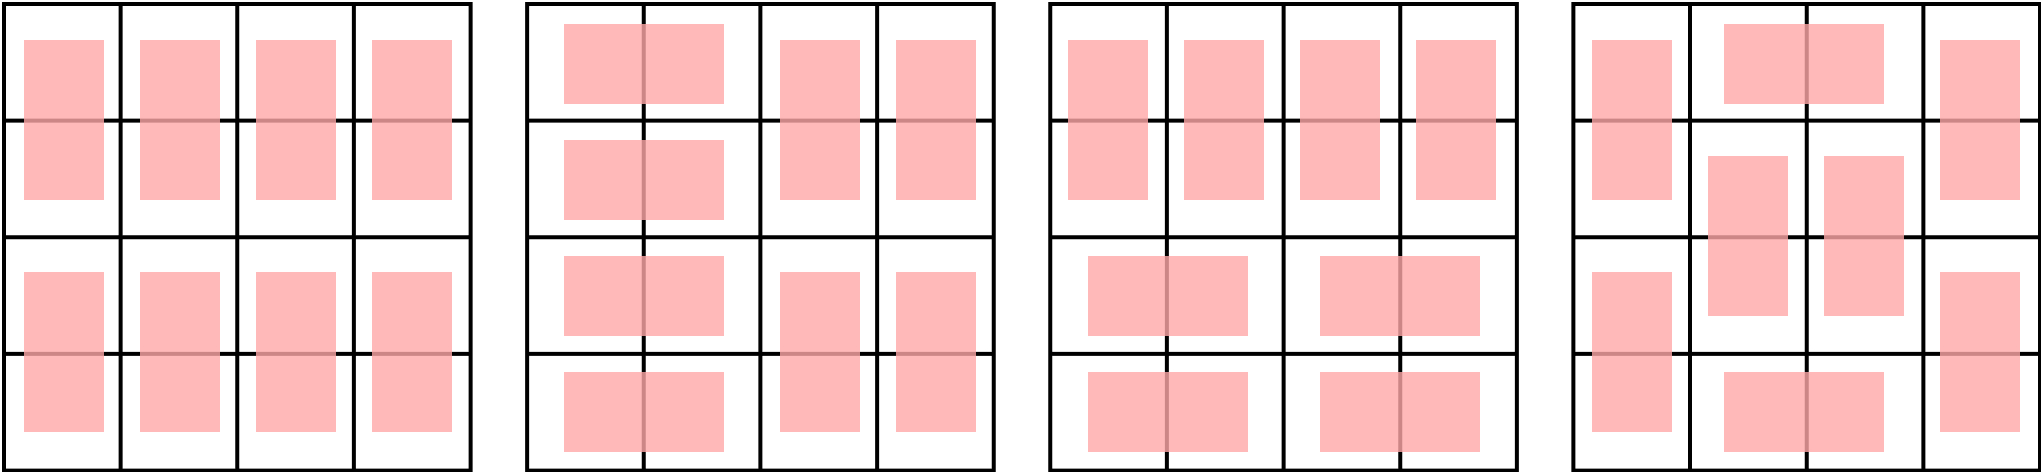
\includegraphics[scale=0.6]{Images/Figure1.jpg}
    \caption{$4$ out of the $36$ possible domino-tilings of a $4\times 4$ board.}
\end{figure}

Next, we state an equivalent formulation of \cref{q:1.7}.

\begin{definition}[Graph]
	A graph is a pair $G=\left( V,E \right)$ where $V$ is a set whose elements are called vertices and $E$ is a set of unordered pairs of vertices whose elements are called edges.
\end{definition}

\begin{definition}[Perfect Matching]
Let $G=\left( V,E \right)$ be a graph. An $M\subseteq E$ is called a perfect matching of $G$ if no two edeges in $M$ share a common vertex and every vertex of $G$ is incident to atleast one edge in $M$.
\end{definition}

\begin{figure}[H]
	\centering
	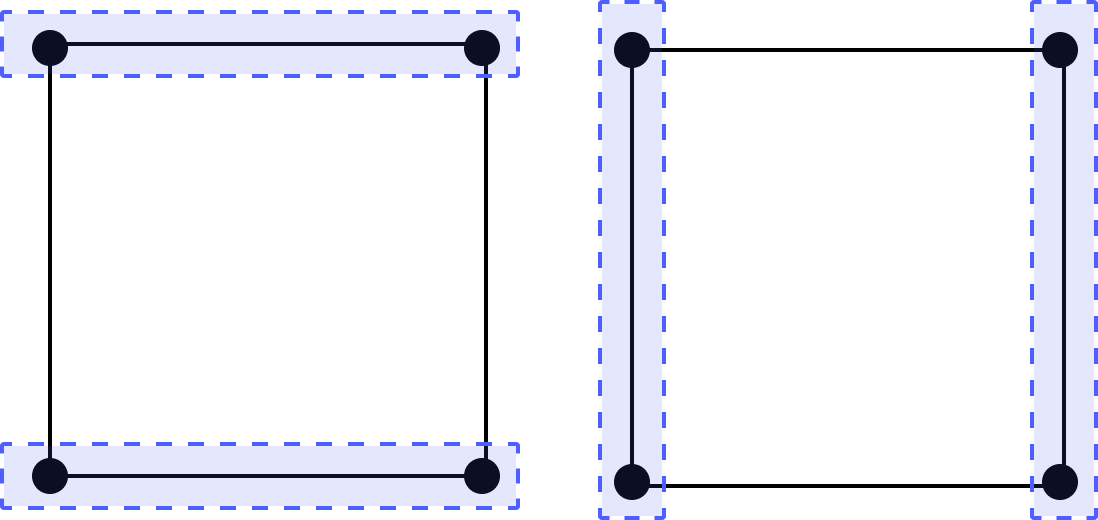
\includegraphics[scale=0.6]{Images/Figure2.jpg}
	\caption{The only possible perfect matchings of the grid graph of order $2$}
\end{figure}
Now consider the following construction. To each square in a given a board of order $m\times n$, we assign a vertex. Additionally, there is an edge between the said vertices if and only if the corresponding squares are adjacent to one another. \cref{f:1.3} is an example of this construction. 

\begin{figure}[H]
	\centering
	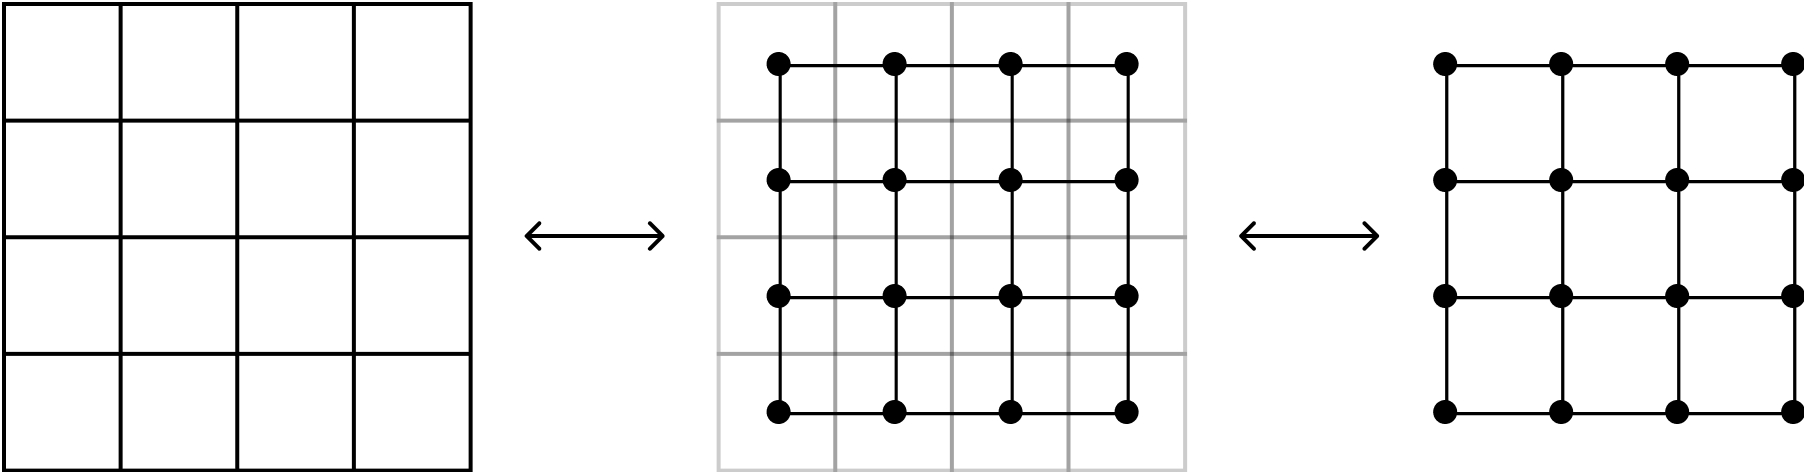
\includegraphics[scale=0.6]{Images/Figure3.jpg}
	\caption{A board of order $4\times 4$ and it's corresponding graph}
	\label{f:1.3}
\end{figure}

It is clear that our construction gives a one-to-one correspondence between the set of possible domino-tilings of a board and the set of perfect matchings of it's corresponding graph.

\begin{figure}[H]
	\centering
	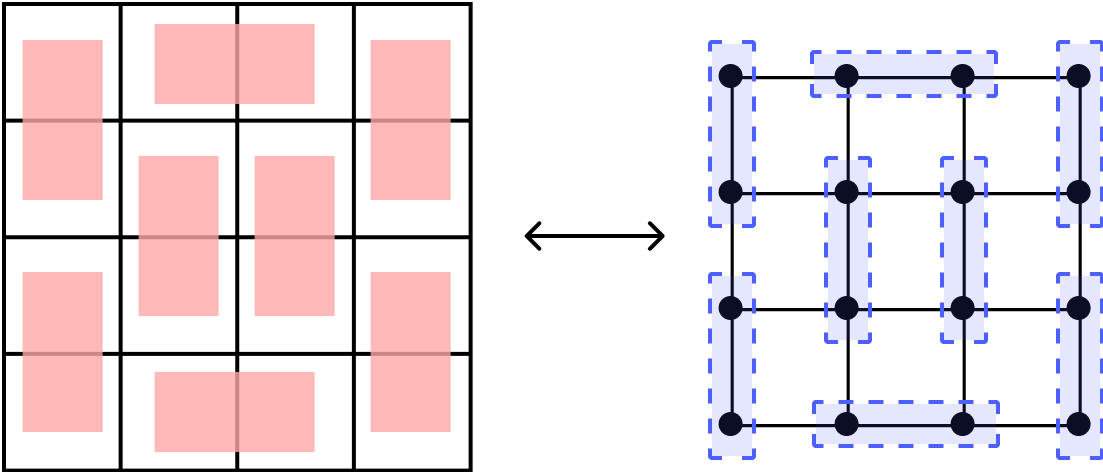
\includegraphics[scale=0.6]{Images/Figure4.png}
	\caption{A domino tiling of a board of order $4\times 4$ and the perfect matching that it admits}
\end{figure}

We shall revisit this formulation of the problem much later in the course. For now, restrict ourselves to a boards of order $2\times n$ and count the number of possible domino tilings, say $t_{n}$ as $n$ varies over the set of natural numbers. It is not too difficult to convince yourself of the fact that $t_{0}=1$, $t_{1}=1$, $t_{2}=2, t_{3}=3$, and $t_{4}=5$. Since the first five terms in the sequence $t_{n}$ are the same as the five terms of the Fibonacci sequence (say $F_{n}$), one might guess that $t_{n} = F_{n}$. This is indeed true, and we shall now give a proof of our claim using a counting argument.
\begin{figure}[H]
	\centering
	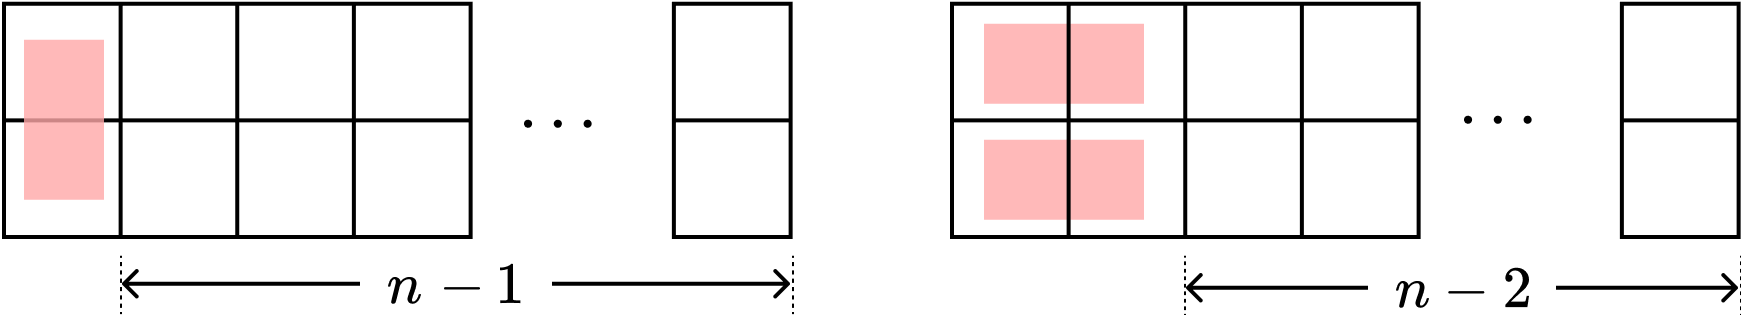
\includegraphics[scale=0.6]{Images/Figure5.png}
	\caption{Two ways to tile the first column of board of order $2\times n$}
	\label{f:1.4}
\end{figure}
\begin{proof}
	Notice how there are exactly two ways to tile the first column of any board of order $2\times n$ (refer to \cref{f:1.4}). It can either be tiled using a single vertical domino, in which case it remains to tile the sub-board of order $2\times \left( n-1 \right)$, or using two horizontal dominos, in which case it remains to tile the sub-board of order $2\times \left( n-2 \right)$. Since both of these cases are valid, it follows that \[
t_{n}=t_{n-1}+t_{n-2}
.\] Which is the same as the Fibonacci reccurence.
\end{proof}

Now that we have $F_{n}=t_{n}$, we prove two standard Fibonacci identities using counting arguments similar to the ones used in the above proof.

\begin{claim}
$F_{m+n}=F_{m}F_{n} + F_{m-1}F_{n-1}$
\label{c:1.1}
\end{claim}

\begin{proof}
\begin{figure}[H]
	\centering
	\begin{subfigure}[b]{0.3\textwidth}
		\centering
		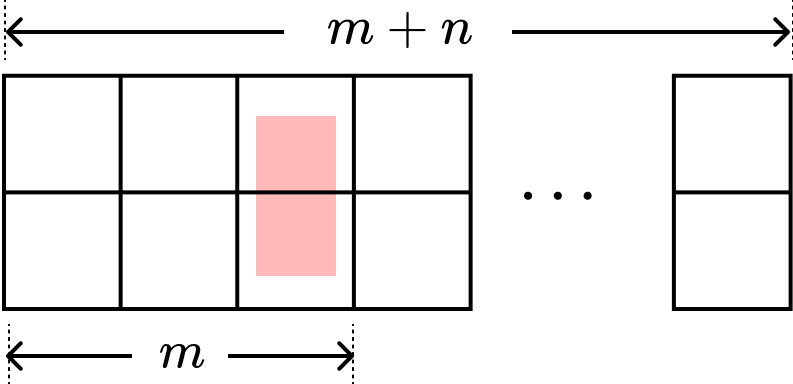
\includegraphics[scale=0.6]{Images/Figure6_1.png}
		\caption{}
	\end{subfigure}
	\hfill
	\begin{subfigure}[b]{0.3\textwidth}
		\centering
		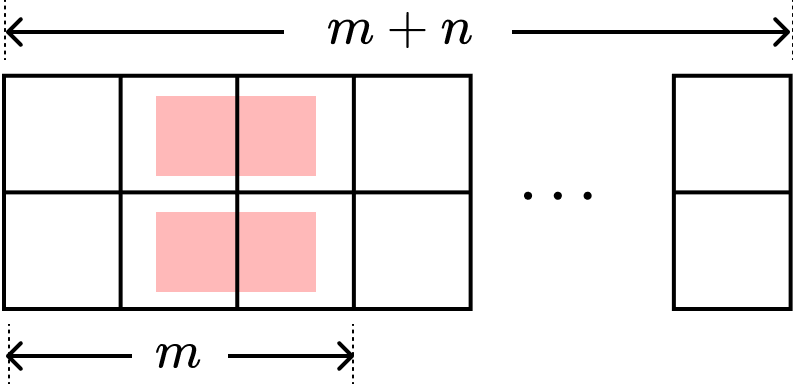
\includegraphics[scale=0.6]{Images/Figure6_2.png}
		\caption{}
	\end{subfigure}
	\hfill
	\begin{subfigure}[b]{0.3\textwidth}
		\centering
		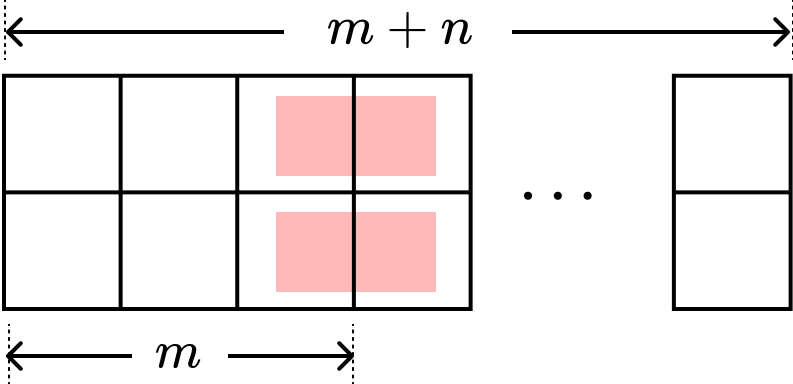
\includegraphics[scale=0.6]{Images/Figure6_3.png}
		\caption{}
	\end{subfigure}
	\caption{The only $3$ ways to tile the $m$-th row of a $2\times \left( m+n \right)$ board.}
	\label{f:1.6}
\end{figure}

Notice how we have exactly $3$ ways to tile the $m$-th row of a $2\times \left( m+n \right)$ board (refer to \cref{f:1.6}). Cases (a) and (b) account for when we have $F_{m}$ ways to tile the sub-block of order $2\times m$ \textbf{and} $F_{n}$ ways to tile the sub-board which occurs immediately after. Case (c), on the other hand, accounts for when we have $F_{m-1}$ ways to tile the sub-board of order $2\times \left( m-1 \right)$ which occurs before the already tiled $m$-th row  \textbf{and} $F_{n-1}$ ways to tile the sub-board of order $2\times \left( n-1 \right)$ which occurs after the already tiled $m$-th row. This proves the required identity.
\end{proof}

\begin{claim}
	$F_{0}+\cdots+F_{n} = F_{n+2}-1$
\end{claim}

\begin{proof}	
Notice how every board of order $2\times k$ has a trivial tiling; the one which only uses vertical dominos and no horizontal ones. On a board of order $2\times \left( n+2 \right)$ if this trivial tiling is ignored, every other possible tiling must have the occurence of atleast one pair of horizontal dominos. If the last such pair occurs at the $n+1$-th column, the sub-board of order  $2\times n$ preceeding it can be tiled in $F_{n}$ ways. If the last such pair occurs at the $n$-th column, the sub-board of order $2\times \left( n-1 \right)$ can be tiled in $F_{n-1}$ ways, and so on. This gives us the required identity. 
\end{proof}
\begin{figure}[H]
		\centering
		\begin{subfigure}[b]{0.3\textwidth}
			\centering
			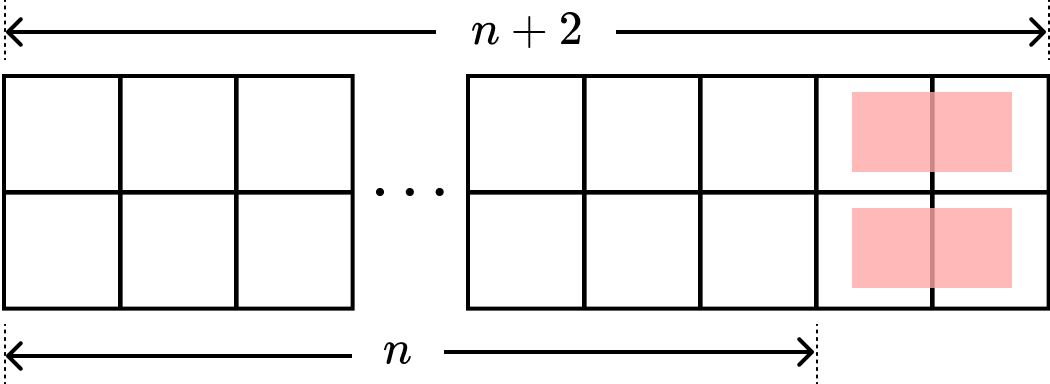
\includegraphics[scale=0.6]{Images/Figure7_1.png}
			\caption{}
		\end{subfigure}
		\vfill
		\begin{subfigure}[b]{0.3\textwidth}
			\centering
			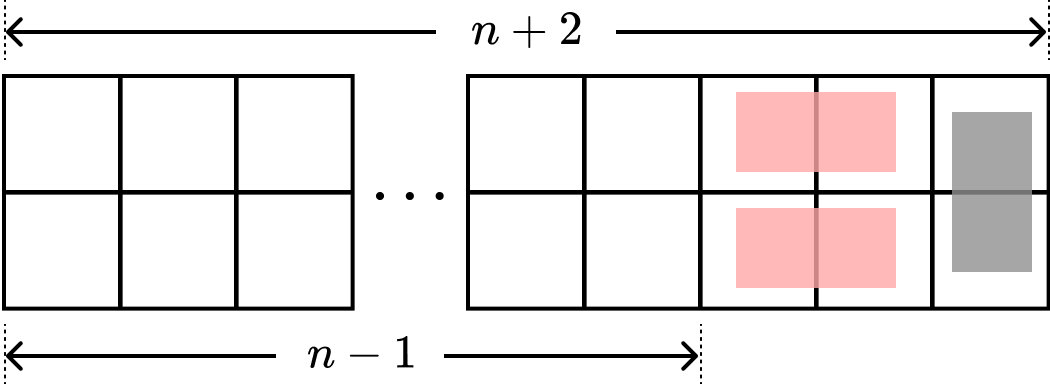
\includegraphics[scale=0.6]{Images/Figure7_2.png}
			\caption{}
		\end{subfigure}
		\vfill
		\begin{subfigure}[b]{0.3\textwidth}
			\centering
			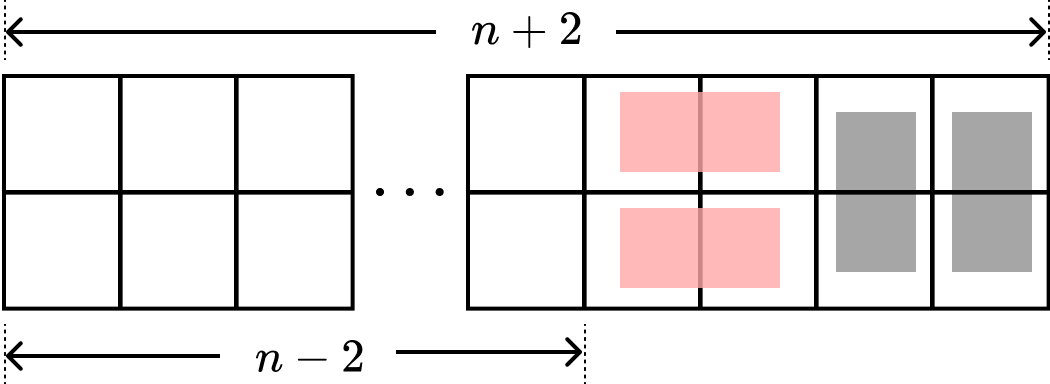
\includegraphics[scale=0.6]{Images/Figure7_3.png}
			\caption{}
		\end{subfigure}
\caption{Examples of occurences of the last pair of horizontal dominos in $3$ non-trivial tilings of a board of order $2\times \left( n+2 \right)$}
\label{f:1.7}
\end{figure}

Recall how $\binom{n}{k}$ counts the number of ways one can choose $k$ elements from a set of $n$ elements. We shall now state a rather interesting re-interpretation of binomial coefficients. 
\begin{figure}[H]
	\centering
	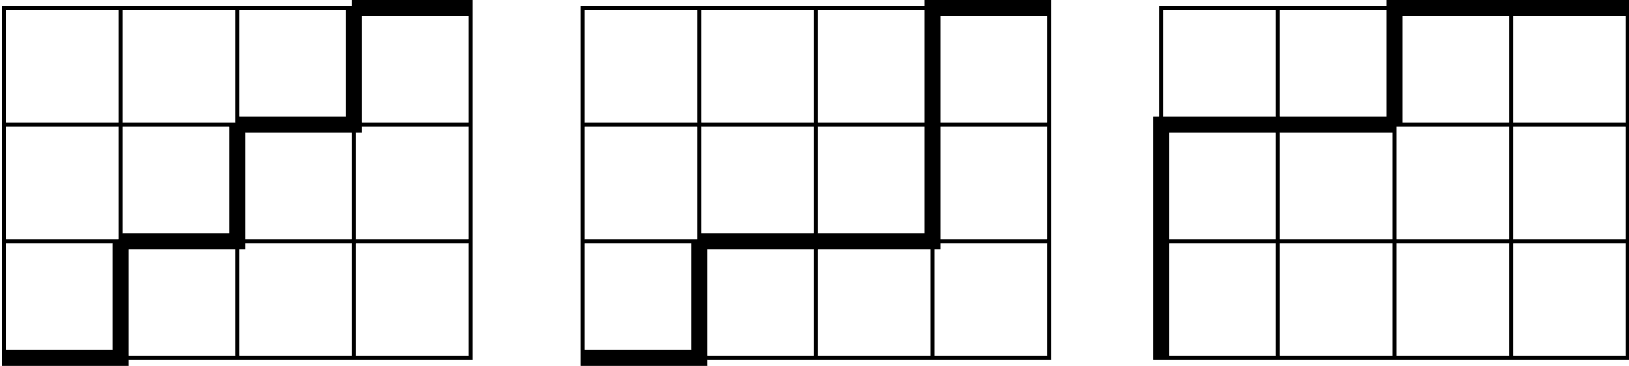
\includegraphics[scale=0.6]{Images/Figure8.png}
	\caption{$3$ examples of lattice paths from $\left( 0,0 \right)$ to $\left( 4,3 \right) $}
	\label{f:1.8}
\end{figure}
\begin{question}
	Given that the only moves allowed are North (N), corresponding to $\left( i,j \right) \to \left( i,j+1 \right)$, or East (E), corresponding to $\left( i,j \right)\to \left( i+1,j \right)$, count the number of paths from $\left( 0,0 \right)$ to $\left( m,n \right)$ on a grid of order $m\times n$ (refer to \cref{f:1.8} for examples of such paths).
\end{question}
Notice how we require exactly $m$ E-moves and $n$ N-moves to reach $\left( m,n \right)$ from $\left( 0,0 \right)$. However, every lattice path is determined completely by a choice of $m$ E-moves (or equivalently $n$ N-moves) which can be made in $\binom{m+n}{m}$ ways (or equivalently $\binom{m+n}{n}$ ways). As a consequence of this counting exercise we have not only given a re-interpretation of binomial coefficients, but have also proved that they are symmetric, i.e, $\binom{n}{k}=\binom{n}{n-k}$.

Per usual, we are now interested in giving a counting argument for a standard identity concerning binomial coefficients called Pascal's identity.
\begin{claim}
	\label{c:1.3}
	$\binom{n}{k} + \binom{n}{k+1} = \binom{n+1}{k+1}$
\end{claim}
\begin{proof}
	Notice how there are $\binom{n+1}{k+1}$ choices of a lattice paths from $\left( 0,0 \right)$ to $\left( n-k,k+1 \right)$. The last step in each one of these paths is either an N-move or an E-move. If it is an N-move then it suffices to choose one lattice path from $\left( 0,0 \right)$ to $\left( n-k-1,k+1 \right)$ out of the \[
		\binom{\left( n-k-1 \right) + \left( k+1 \right)}{k+1} = \binom{n}{k+1}
	\] choices. Alternatively, if it is an E-move then it suffices to choose one lattice path from $\left( 0,0 \right)$ to $\left( n-k,k \right)$ out of the \[
	\binom{\left( n-k \right) + k}{k} = \binom{n}{k}
	\] choices.
\end{proof}

Let's remind ourselves that the central objective of this course is to count. From \cref{q:1.1} through \cref{q:1.6}, we encountered examples where we derived exact closed-form expressions for counting. During our discussion of the dimer model, we first stated a closed-form expression and then constructed a bijection between the tiling configuration and the perfect matchings configuration. By restricting ourselves to boards of size $2 \times n$, we demonstrated that finding a recurrence relation is also a valid counting technique. However, as we will see, the methods we have discussed so far are not always applicable. In such cases, we turn to the idea of generating functions, which we will introduce next.

\begin{definition}[Generating Function]
	Given a sequence $\{a_{n}\}_{n \ge 0}$ the formal power series, $\sum_{k=0}^{\infty}a_{k}x^k$, in an indeterminate $x$ is called the generating function of $\{a_{n}\}_{n \ge 0}$.
\end{definition}

Since our definition works with a \textit{formal} power series we need not worry about the divergence of the involved infinite sum. That being said, we can always be cautious and assume $|x|<1$ to guarantee convergence. 

\begin{question}
	Find the generating function for the sequence of Fibonacci numbers 
\end{question}
Let $\{f_{n}\}_{n \ge 0}$ denote the sequence of Fibonacci numbers and let $F\left( x \right)$ be the corresponding generating function. Notice how 
\begin{align*}
	F\left( x \right) &= \sum_{k=0}^{\infty} f_{k}x^k \\
	&= f_{0}+f_{1}x+\sum_{k=2}^{\infty}f_{k}x^k \\
	&= 1+x+\sum_{k=2}^{\infty}f_{k}x^k \\
	&= 1+x+\sum_{k=2}^\infty \left( f_{k-1}+f_{k-2} \right) x^k \\
	&= 1+x+\sum_{k=2}^{\infty} f_{k-1}x^k + \sum_{k=2}^{\infty} f_{k-2}x^k \\
	&= 1+x+x\left( F\left( x \right) -1 \right) + x^2F\left( x \right)  \\
	&= 1+xF\left( x \right)+x^2F\left( x \right)
\end{align*}
Solving which we obtain \[
F\left( x \right) = \frac{1}{1-x-x^2}
\].

Throughout this course, we will explore how and why generating functions are extensively used in combinatorics. We introduce one such instance now, which will be discussed in greater depth later.

\begin{definition}
An integer partition of a natural number $n$ is a non-increasing sequence of natural numbers, $\{\lambda_i\}_{i \ge 1}$, whose sum is $n$.
\end{definition}

\begin{question}
In how many ways can a natural number $n$ be partitioned?
\end{question}

Let $p(n)$ denote the number of partitions of $n$. Interestingly, no "nice" closed-form expression for $p(n)$ has been found. However, we will derive the generating function \[
	\prod_{n=1}^\infty\left( 1+x^n +x^{2n}+x^{3n}+\cdots\right) =  \sum_{n=0}^{\infty}p\left( n \right) x^n
\] which was given by Euler, later in the course.

\begin{remark}
	In the year 1918, G.H Hardy and Srinivasa Ramanujan obtained an asymptotic expression (an expression which describes the limiting behaviour) for $p\left( n \right)$ which is given by \[
	p\left( n \right) ~ \frac{1}{4n\sqrt{3}}\exp\left( \pi \sqrt{\frac{2n}{3}}  \right) 
	.\] Oftentimes stating an asymptotic expression is also a valid counting technique.
\end{remark}

\section{Counting Principles}
We state the fundamental counting principles now.
\begin{enumerate}
\item (Addition Principle): If $\{A_{k}\}_{k\geq 1}$ is a family of finite and pairwise disjoint sets then $\abs{\bigcup_{k\geq 1} A_{k}} = \sum_{k\geq 1}\abs{A_{k}}$.
\item (Substraction Principle): If $A$ and $B$ are finite sets such that $B\subseteq A$ then $\abs{A\backslash B} = \abs{A}-\abs{B}$.
\item (Product Rule): If $A$ and $B$ are finite sets, then $\abs{A\times B} = \abs{A}\cdot\abs{B}$.
\item (Division Rule): For finite sets $A$ and $B$ if there exists a $d$-to-many function $f:A\to B$ then $\abs{B}=\abs{A}/d$.
\end{enumerate}
In some sense we've already been using these principles in disguise thus far. For instance;

\begin{question}
	How many $k$-digit positive numbers are there?
\end{question}
Since we have $10$ choices for the first $\left(k-1\right)$ digits and $9$ choices for the last digit, by the product rule there are $9\cdot 10^{k-1}$ $k$ digit numbers.


This is a good point to recall the binomial theorem and prove it using a counting argument instead of the standard induction argument.

\begin{theorem}[Binomial Theorem]
	\[
		\left( x+y \right)^n = \sum_{k=0}^{n}\binom{n}{k}x^{n-k}y^k
	.\] 
\end{theorem}
\begin{proof}
	Consider the expansion of
	\[
		\left( x+y \right)^n = \underbrace{\left( x+y \right) \cdots \left( x+y \right) }_{n \text{ factors}}.
	\]
	In this expansion, there are $\binom{n}{k}$ ways to choose $x$ from exactly $k$ of the $n$ factors (which forces the choice of $y$ from the remaining $(n-k)$ factors). Since $k$ can range from $0$ to $n$, applying the addition principle gives us the binomial theorem.
\end{proof}
Now we state a the multinomial theorem which generalizes the binomial theorem to expressions with more than two terms, allowing us to expand any power of a sum of multiple terms as a sum of products of those terms, each multiplied by a what is called a multinomial coefficient which is denoted and defined as
\[\binom{n}{k_1,\cdots,k_m} := \frac{n}{k_1!\cdots k_m!}.\]
We would expect the multinomial coefficient to count something. That is indeed the case, it counts the number of ways to arrange $n$ distinct objects into $m$ distinct bins such that the $i$-th bin contains $k_i$ elements. With this interepretation of multinomial coefficients, mimicing the steps involved in the proof of the binomial theorem we get the multinomial theorem which is stated below. 
\begin{theorem}[Multinomial Theorem]
	\[
	(x_{1}+\cdots+x_{r})^n = \sum_{k_{1}+\cdots+k_{r}=n}\binom{n}{k_{1},\cdots,k_{r}}x_{1}^{k_{1}}\cdots x_{r}^{k_{r}}
	.\] 
\end{theorem}
It is natural to expect a Pascal-like identity for multinomial coefficients as well. In this spirit consider the following claim.
\begin{claim}
	\[
		\binom{n}{k_{1},\cdots,k_{r}} = \binom{n-1}{k_1-1,k_2,\cdots,k_r} + \cdots + \binom{n-1}{k_1,k_2,\cdots,k_r-1}
	.\]
\end{claim}
\begin{proof}
\end{proof}
Notice how when $k_1=k$, $k_2=n-k$ and all the other $k_i$s are $0$, we retrieve the Pascal's identity (\cref{c:1.3})
\begin{comment}
	
Generalization of the binomial theorem to the binomial theorem which is the multinomial theorem. Explain the multinomial coefficient here first.
	Then show that 
	\begin{claim}
		\binom{n}{k_{1},\cdots,k_{r}} = \binom{n}{k_{1}}\binom{n-k_{1}}{k_{2}}\binom{n-k_{1}-k_{2}}{k_{3}} \cdots \binom{n-k_{1}-\cdots-k_{m-1}}{k_{r}}
	\end{claim}
	and finally give a proof of
Proof is similar to the proof of the binomial theorem.

Proof involves rewrriting $(x_{1}+\cdots+x_{r})^n$ as $(x_{1}+\cdots+x_{r})(x_{1}+\cdots+x_{r})^{n-1}$ and then swapping the two sums. Change of variables. And we're done.
\end{comment}

In addition to the fundamental counting principles, there are a few more principles/techiniques which we will use quite often in this course. One of them is the bijection principle. We state the principle formally and then given an example.

\begin{theorem}[Bijection Principle]
If $S$ and $T$ are finite sets then $|S|=|T|$ if and only if there exists a bijection $f:S\to T$.
\end{theorem}
 
\begin{question}
	Let $S$ be a finite set. A \textbf{permutation} of $S$ is a bijection from and to $S$. How many permutations of $[n]=\{1,2,3,\ldots,n\}$ exist?
\end{question}

We introduce the cycle notation before outlining a solution. In the case where $n=1$, it is clear that there is only possible bijection, namely, $f_1:\{1\}\to\{1\}$ such that $f_1 \left(1 \right) =1$. We shall write $f_1$ as \[
\begin{pmatrix}
	1 \\ 1
\end{pmatrix}
.\] In the case where $n=2$, it is clear that there are two possible bijections. These are $g_1:\{1,2\}\to \{1,2\}$ such that $g_1\left(1 \right) =1$, $g_1\left( 2 \right)=2$, and $g_{2}:\{1,2\}\to\{1,2\}$ such that $g_{2}\left(1  \right) =2$, $g_{2}\left( 2 \right) =1$. We shall write $g_{1}$ and $g_{2}$ as \[
\begin{pmatrix} 1 & 2 \\ 1 & 2 \end{pmatrix}, \quad \begin{pmatrix} 1 & 2 \\ 2 & 1 \end{pmatrix} 
\] respectively. In essence, the first row in our notation lists the elements of the domain, and the second row lists where the bijection sends these elements. Do you see why in the case where $n=3$ the bijections can be written as 
 \[
	 \begin{pmatrix} 1 & 2 & 3 \\ 1 & 2 & 3 \end{pmatrix}, \begin{pmatrix} 1 & 2 & 3 \\ 1 & 3 & 2 \end{pmatrix}, \begin{pmatrix} 1 & 2 & 3 \\ 2 & 1 & 3 \end{pmatrix}, \begin{pmatrix} 1 & 2 & 3 \\ 2 & 1 & 3 \end{pmatrix}, \begin{pmatrix} 1 & 2 & 3 \\ 2 & 3 & 1 \end{pmatrix}, \begin{pmatrix} 1 & 2 & 3 \\ 3 & 1 & 2\end{pmatrix}, \begin{pmatrix} 1 & 2 & 3 \\ 3 & 2 & 1 \end{pmatrix} 
.\]
Since the first row of any bijection in our notation is fixed and we have \[ n\cdot\left( n-1 \right) \cdots 1 = n!\] ways to fill out the second row, it clear that there are $n!$ permutations of $[n]$. Recall from \cref{q:1.5} that we also have exactly $n!$ permutation matrices. By the bijection principle we must have a bijection between the set of permutation matrices of order $n\times n$ and the set of permuations of $[n]$. The bijection is as follows. Corresponding to every permutation \[
\begin{pmatrix} 
	1 & 2 & \cdots & n \\
	f\left(1\right) & f\left( 2 \right) & \cdots & f\left( n \right)
\end{pmatrix} 
\] of $[n]$ we assign an $n\times n$ matrix where the entry at $\left( i,f\left(i  \right)  \right)$ for $1\leq i\leq n$ is $1$, and all other entries are $0$. More explicity,
\begin{align*}
    &\begin{pmatrix}
    1 & 2 & 3 \\
    1 & 2 & 3 
\end{pmatrix}
\longleftrightarrow
\begin{pmatrix}
    1&& \\
    &1& \\
    &&1
\end{pmatrix}, \\
&\begin{pmatrix}
    1 & 2 & 3 \\
    1 & 3 & 2 
\end{pmatrix}
\longleftrightarrow
\begin{pmatrix}
    1&& \\
    &&1 \\
    &1&
\end{pmatrix}, \\
&\hspace*{6em}\vdots \\
&\begin{pmatrix}
    1 & 2 & 3 \\
    3 & 2 & 1
\end{pmatrix}
\longleftrightarrow
\begin{pmatrix}
    &&1\\
    &1&\\
    1&&
\end{pmatrix}.
\end{align*}
We outline a proof of an identity involving binomial coefficients using the bijection principle now.
\begin{claim}
\begin{align*}
\sum_{i=0}^{n}\binom{n}{i} = 2^n
\end{align*}
\label{c:2.1}
\end{claim}
\begin{proof}
	Let \( S = \{a_1, \ldots, a_n\} \) be a set with \( n \) elements. For each of the \( 2^n \) possible subsets \( T = \{a'_1, \ldots, a'_k\} \) of \( S \) (where \( k \) can be any value from 0 to \( n \)), there is a corresponding binary string of length \( n \). In this string, the \( i \)th bit is \( 1 \) if the element \( a_i \) is in the subset \( T \), and \( 0 \) if it is not. For instance in the case where $S=\{0,1\}$ we have the following correspondence
	 \begin{align*}
		&\emptyset \longleftrightarrow 00 \\
		&\{0\} \longleftrightarrow 10 \\
		&\{1\} \longleftrightarrow 01 \\
		&\{0,1\} \longleftrightarrow 11
	\end{align*}
\end{proof}
Another counting technique which we've seen before in the proof of Pascal's identity (\cref{c:1.3}) is called double counting. The broad idea is to count the same combinatorial object in two different ways. As an example, we give a proof of \cref{c:2.1} using the double counting technique.
\begin{proof}
It is clear that $2^n$ counts the number of $n$-bit binary strings. To prove the claimed identity, we count the number of $n$-bit binary strings once again in a different way. Notice how an arbitrary$n$-bit binary string has $0\leq i\leq n$ number of $0$s. Since there are $\binom{n}{0}$ choices when $i=0$, $\binom{n}{1}$ choices when $i=1$, and so on, by the addition principle we have proved the required identity.
\end{proof}

We have all seen a proof by induction of the following identity. Now we give a proof using a double counting argument.
\begin{claim}
	$1+2+3+\cdots+n=\dfrac{n\left( n+1 \right)}{2}=\binom{n+1}{2}$
	\label{c:2.2}
\end{claim}
\begin{proof}
	Consider the problem of counting the number of handshakes in a group of $n+1$ people, where each person shakes hands with every other person. The first person in the group shakes hands with everyone except themselves; this gives $n$ handshakes. The second person in the group shakes hands with everyone else; this gives $\left( n-1 \right)$ handshakes (not $n$ because we've already counted the handshake between the first and second person). The third person in the group shakes hands with everyone; this gives $\left( n-2 \right)$, and so on. In all we have $n+\left( n-1 \right)+\left( n-2 \right)+\cdots+1$ handshakes. Let's count again in a different way now. Notice how for each pair of people there is one handshake. Hence, there are $\binom{n+1}{2}$ handshakes in total. Putting the two observations together proves the claim.
\end{proof}

Next, we introduce the ``stars and bars'' method. We shall outline how this method works with the help of a few standard examples.
\begin{question}
	For a given $n\in \mathbb{N}$ how many $x_{1},\cdots,x_{r}\geq 0$ exist which add upto $n$?
\end{question}

\begin{comment}
https://math.stackexchange.com/questions/2018957/number-of-solutions-to-x-1x-2-x-m-n
||||+||+| and so on. So we're just making a choice of the number of +s

\end{comment}

We conclude this section by stating an informal technique called proof by pictures (or proof without words). This technique involves the use of visual representations to demonstrate the validity of a mathematical statement. Although in the strictest sense of things a proof by pictures is not a counting principle, it often helps develop intution. For instance, we state such a proof for \cref{c:2.2}. 
\begin{proof} 
	\begin{figure}[H]
		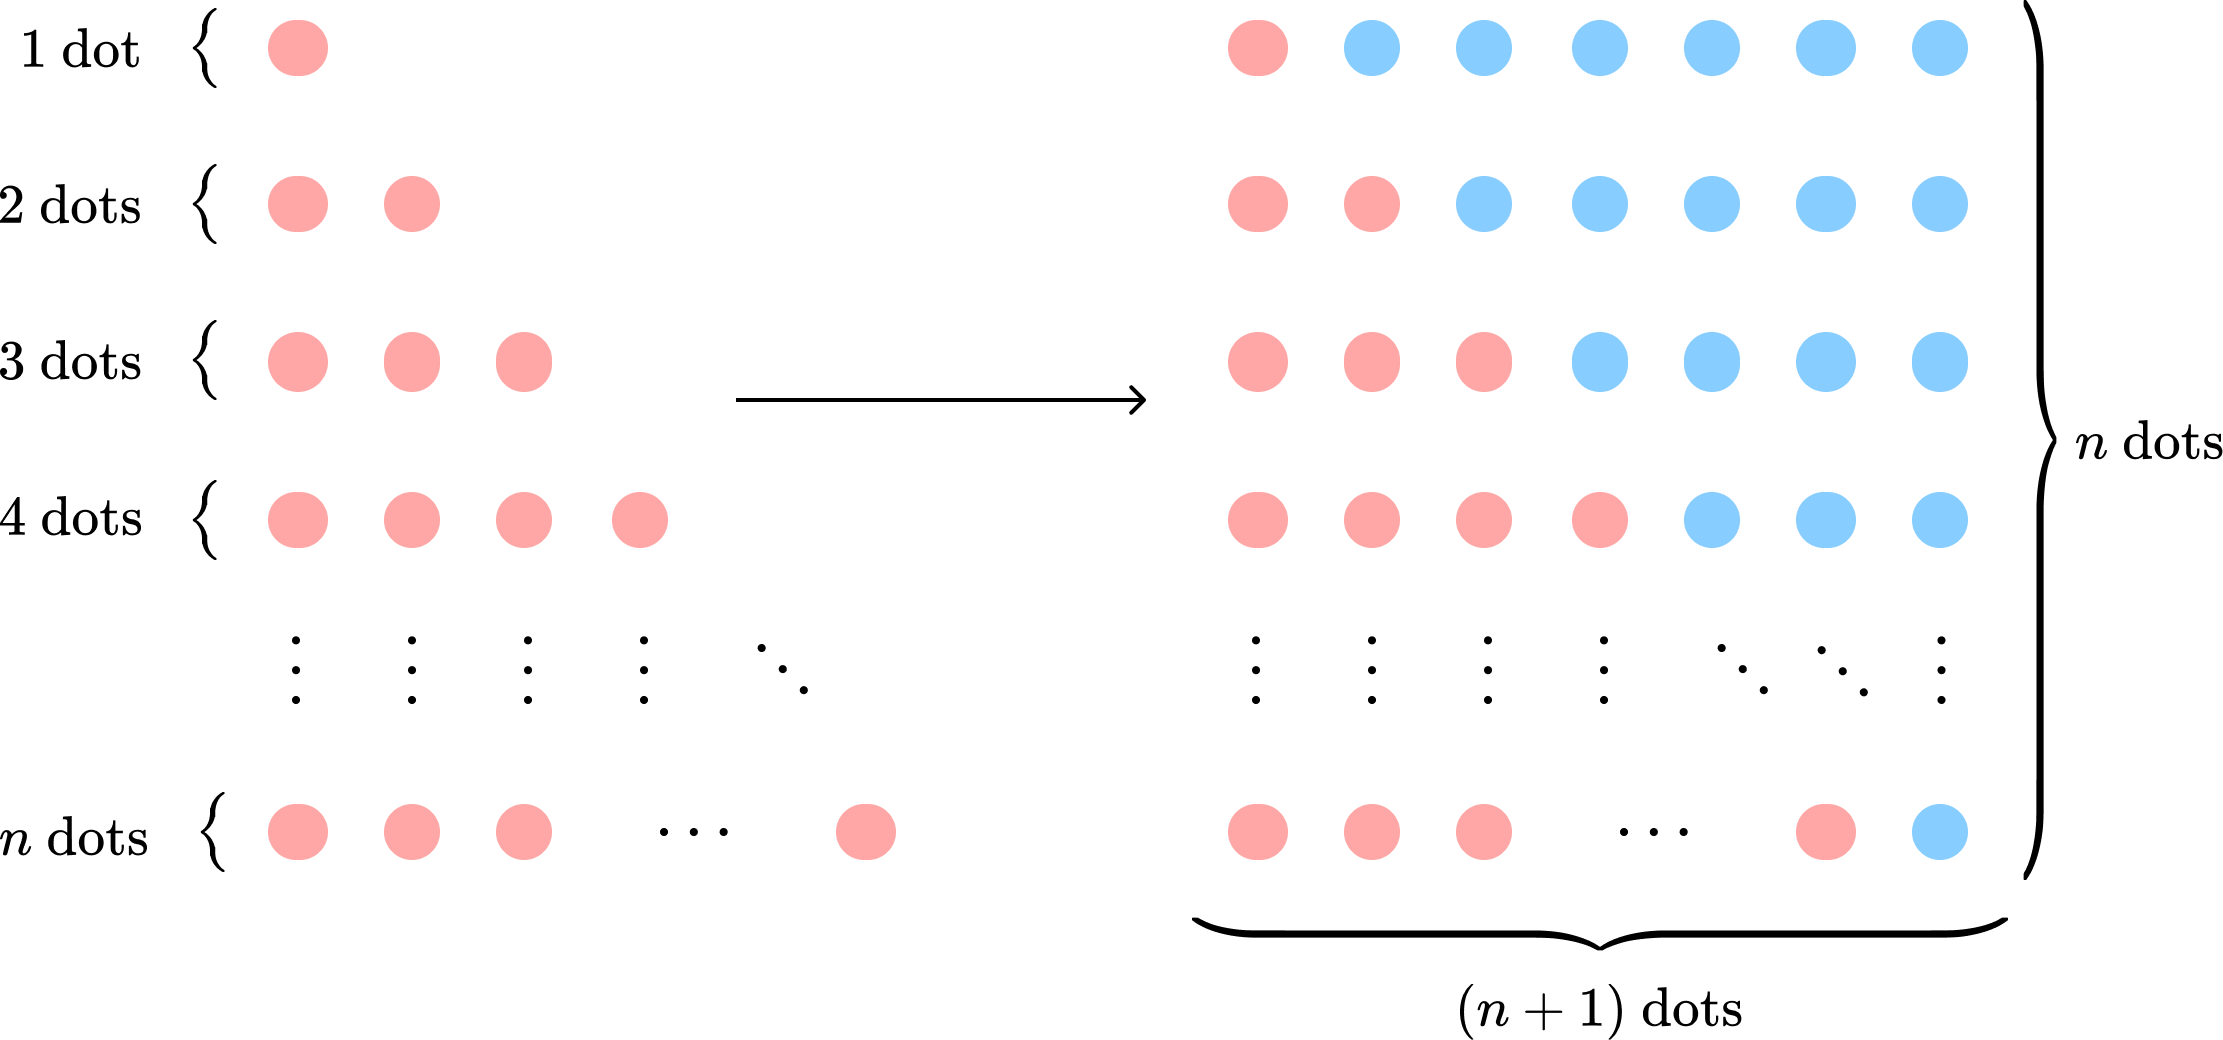
\includegraphics[scale=0.65]{Images/Figure9.png}
		\caption{}
		\label{f:1.9}
	\end{figure}
In \cref{f:1.9} notice how there are $1+2+3+\cdots+n$ dots colored in red, $1+2+3+\cdots+n$ dots colored in blue, and hence $2\left( 1+2+3+\cdots+n \right)$ total. It is also true that in our arrangement there are $n\left( n+1 \right)$ dots in total. Now the identity follows.
\end{proof}
Yet another fundamental counting principle is the pigeonhole principle. Given its importance, we will dedicate the upcoming section to explore it in detail.
\begin{remark}
We have seen how the principles we’ve discussed so far can be useful in proving combinatorial identities. Determining how to derive these identities is not always straightforward. However, a common technique involves running computer simulations to generate a sequence of values corresponding to the first few natural numbers. Tools like OEIS, RATE (in Mathematica), and Guess (in SageMath and Maple) can then be used to conjecture a closed form for the sequence.
\end{remark}

\begin{comment}
-------
Challenge problems:
-----
$t_{n} = \binom{n}{0}+\binom{n-1}{1}+\binom{n-2}{2} + \cdots$
$\binom{2n}{n} = \sum_{k=0}^{n}\binom{n}{k}^2$

Consdier a $4 x 4$ chessboard. We want to place as many queens as possible such that they don't attack each other. What are the possible number of such configurations. What are the maximum number of queens you can place? Show that it has to be less than $5$. Give two examples of configurations with $4$ queens. This works only for chessboard greater than $4$ (i.e order n and n queens).

We want to find the number of solutions to the equation $x_{1}+\cdots+x_{k}=n$ where $n\in\mathbb{N}$ and  $x_{i}\in\mathbb{Z}$. We have the following cases:
	\begin{enumerate}
		\item All $x_{i}>0$: How many compositions of $n$ into $k$ parts
		\item All $x_{i}\geq 0$ : What are the monomials of degree $n$ in  $k$ variables
	\end{enumerate}

	Compositions are partitions where the order matters.
	Weak compositions are compositions in which $0$ is allowed.

	We are given  $n$ balls which we want to arrange into  $k$ compartments. In the first case we are not allowed to have empty compartmenets, in the other case it's allowed. 
	We just want to choose $k-1$ boundaries out of the  $n+k=1$ objects which is just  $\binom{n+k-1}{k-1}$ (CASE B)

	$\binom{n-1}{k-1}$ (CASE A)

	There is also a proof using generating functions which we shall discuss in the upcoming sections
\end{comment}

\section{The Pigeon-hole Principle}
We state what is known as the pigeon-hole principle.
\begin{theorem}
Let $A_{1},\cdots,A_{k}$ be pair-wise disjoint finite sets. If \[|A_{1}\cup A_{2}\cup \cdots \cup A_{k}|>kr\] then there exists an $1\leq i\leq k$ such that $|A_{i}|>r$.
\end{theorem}
Even though the statement sounds trivial, it has immense applications. We state a few examples now. 
\begin{claim}
Given $b\in \mathbb{Z}$, the decimal expansion of $1/b$ is either finite or eventually periodic.
\end{claim}
\begin{proof}
Each step in the long division of $1$ by $b$ involves subtracting multiples of $b$ from powers of $10$ until the remainder is $0$ or repeats itself. Since each one of these remainders must be strictly less than $b$, we have $b$ possible remainders, namely, $0, 1, 2, \cdots, b-1$. If the remainder becomes $0$ at some step, the division terminates, in which case the decimal expansion is finite. Next, consider the case where the division does not terminate. By the pigeon-hole principle, since there are only $b$ possible remainders and more than $b$ steps, at least one of the remainders must repeat. This proves our claim because when a remainder repeats, the sequence of digits that follow in the decimal expansion must repeat as well.
\end{proof}
\begin{claim}
Let $S=\{1,2,\cdots,2n\}$. Any $n+1$ element subset $K$ of $S$ has two numbers $a$ and $b$ such that
\begin{enumerate}
	\item $\gcd(a,b) = 1$
	\item $a=nb$ for some $n\in\mathbb{N}$
\end{enumerate}
\end{claim}
\begin{proof}
\begin{enumerate}
\item Consider the $n$-element subset \[\{\left( 1,2 \right), \left( 3,4 \right), \cdots \left( 2n-1,2 \right)\}\] of $S\times S$ and notice how if we choose $n+1$ numbers from $\{0,\cdots,2n\}$ then by the pigeonhole principle we are guaranteed to pick two numbers from the same pair in $S\times S$. Since each element in the said subset is a pair of consecutive numbers, their $\gcd$ is necessarily $1$.
\item Notice how every element in the set $\{1,2,\cdots,2n\}$ can be written in the form $2^ab$ where $b$ is odd by factoring out as many $2$s as possible. Since there are only $n$ odd numbers in these set $\{1,2,\cdots,2n\}$, we are left with $n$ choices of $b$. Next, we construct $b$ subsets of $S$, say $S_k\subseteq S$ such that $i\in S_k$ if and only if $i=2^kb$. Finally, by the pigeonhole principle, if one were to pick $n+1$ elements from $S$ atleast $2$ of them would be in the same $S_k$, i.e, there always exists a pair of numbers such that one divides the other.
\end{enumerate}
\end{proof}
\begin{claim}
If $S$ be an $n+1$-element set of natural numbers, then there exists a pair of numbers in $S$ whose difference is divisible by $n$.
\end{claim}
\begin{claim}
Given $m$ integers say  $a_{1},\cdots,a_{m}$ prove that there exists $k$ and $l$ with  $0\leq k\leq l\leq m$ such that $m$ divides  $a_{k+1}+a_{k+2}+\cdots+a_{l}$
\end{claim}
\begin{claim}
In a party of $n$ people, where some (maybe all, maybe none) shake hands with one another, show that there are atleast two people who shake the same number of hands.
\end{claim}
\begin{claim}
In a group of $6$ people where each pair of people are either friends or enemies, show that there are  $3$ people who are either all friends or all enemies. 
\end{claim}
\begin{comment}
Give a normal explanation. and the graph theoritic approach. 
\[
	\sum_{v\in V}degree(v) = 2|E|
.\] 
Introduce Ramsey's theorem
\end{comment}
We conclude this section by stating a few definition which will turn out to be useful in the upcoming sections.
\begin{definition}[$k$-Permutation]
A $k$-permutation on $[n]=\{1,2,\cdots,n\}$ is a bijection between two $k$-element subsets of $[n]$. 
\end{definition}
\begin{definition}[Circular $k$-Permutation]
	$k$-permutations  $\pi$ and $\sigma$ are called circular equivalents if there exists a shift  $s\in [k]$ such that  $i+s\equiv j(\text{mod} \ k)$.
\end{definition}
\section{The Principle of Inclusion-Exclusion}
Recall that for finite sets $A$ and $B$, the cardinality of their union is given by $|A \cup B| = |A| + |B| - |A \cap B|
$. This formula, which adds (includes) the sizes of $A$ and $B$ while subtracting (excluding) the overcount in $|A \cap B|$ encapsulates the essence of the inclusion-exclusion principle. We start with a useful generalization of the motivating formula we just discussed.
\begin{theorem}
	Given finite sets $A_{1},\cdots,A_{k}$, 
	\[
		|\bigcup_{i=1}^k A_i| = \sum_{n=1}^{k}\left(-1  \right)^{n+1}\left( \sum_{1\leq i_{1}<\ldots<i_{n}\leq k+1}|A_{i_{1}}\cap \cdots A_{i_{n}}| \right) 
	.\] 
\end{theorem}


\chapter{The Art of Combinatorial Thinking}
\section{Binomial Coefficients}
This section aims to push-forward our familiarity with binomial coefficients which we have gained from the previous chapter. We do so by outlining proofs of a few standard combinatorial identities.
\begin{comment}
Three numbers out of the $n+1$ choices say $a_{1}<a_{2}<a_{3}$. Now argue for the first three sums based on which one of these is chosen first. 

The first sum corresponds to choosing $a_2$. The second sum corresponds to choosing  $a_{3}$. The third sum corresponds to choosing $a_{1}$.

\begin{question}
	For all $n\geq r\geq 0$ we have 
	 \[
		 \binom{r}{r}+\binom{r+1}{r}+\cdots+\binom{n}{r} = \binom{n+1}{r+1}
	.\] 
\end{question}
Give a proof using lattice paths. 
RHS is the number of lattice paths from $(0,0)\to (r+1,n-r)$. For the LHS what happens before the last E step.

The idea is not always to prove equalities. Infact more often than not we will be interested in proving inequalities
 \begin{question}
	 \binom{2n}{n}<4^n
\end{question}
Convert binary to lattice: 0 to N, 1 to E and so on.

\begin{question}
	For all $n>0$. \[
		\sum_{k=0}^{n} 2^k\binom{n}{k} = 3^n
	\]
\end{question}

\begin{question}
	For $n>0$  \[
		2\binom{2n-1}{n} = \binom{2n}{n}
	.\] 
\end{question}
Give two proofs. One using Pascals identity. The other by choosing sets.
\end{comment}

\begin{claim}
\[
\sum_{k=1}^{n}k\binom{n}{k}^2 = n\binom{2n-1}{n-1}
\]
\end{claim}
\begin{proof}
Let $J$ be a collection of $2n$ objects which is partitioned into $2$ equal sub-collections $J_1$ and $J_2$. Now, we want to make a choice of $n$ elements from $J$ which includes a distinguished element, say $x$ from $J_1$ (or equivalently $J_2$). Since there are $n$ ways to choose the said distinguished element, and $\binom{2n-1}{n-1}$ ways to choose the rest of the $n-1$ elements, in all we have \[
n\binom{2n-1}{n-1}
\] ways to make the said choice. Alternatively, we can also choose $k$ elements from $J_1$ in $\binom{n}{k}$ ways, $n-k$ elements from $J_2$ in $\binom{n}{n-k}$ ways, and then choose the distinguished element from $J_1$ (or equivalently $J_2$) in $1\leq k\leq n$ ways. Thus far, we have proved
\[
\sum_{k=1}^{n}k\binom{n}{k}\binom{n}{n-k} = n\binom{2n-1}{n-1}.
\]
Since by \cref{r:1.2} \[
\binom{n}{k} = \binom{n}{n-k},
\]
we are done. 
\end{proof}
\begin{claim}
\[
\sum_{k=1}^{n}k\binom{n}{k} = n2^{n-1}
\]
\end{claim}
\begin{proof}
In a class of $n$ students, a football coach wants to choose students to form a football team of $1\leq k\leq n$ players. Additionally, the coach also wants one of $k$ students to be the captain of the team. Since the representative can be chosen in $n$ ways and the remaining set of students can be chosen in $2^{n-1}$ ways, the team can be chosen in $n2^{n-1}$ ways.  Alternatively, the coach can select $k$ players out of $n$ in $\binom{n}{k}$ ways, and then choose the captain in $k$ ways. Since $0<k\leq n$, we are done. 
\end{proof}

\begin{claim}
\[
\sum_{i=1}^{n}i(n-1) = \sum_{i=1}^{n}\binom{i}{2} = \sum_{i=0}^{n-2}\binom{n-i}{2} = \binom{n+1}{3} 
\]
\end{claim}
\begin{proof}
It is clear that $\binom{n+1}{3}$ is the number of ways to choose $3$ numbers, say $a_{1}<a_{2}<a_{3}$, from the $n+1$-element set $\{a_1,\cdots,a_{n+1}\}$. Now we argue based on which one of these three is chosen first. If 
\end{proof}
\begin{claim}
For all $n\geq r\geq 0$ we have 
\[
\binom{r}{r}+\binom{r+1}{r}+\cdots+\binom{n}{r} = \binom{n+1}{r+1}
.\] 
\end{claim}
\begin{proof}
We give a double counting argument. Noitce how $\binom{n+1}{r+1}$ counts the number of ways to choose $(r+1)$-element subsets of $[n+1]=\{1,\ldots,n+1\}$. A choice of the said subsets can also be made by first fixing the largest of the $r+1$ numbers. This is given by $\binom{r}{r}+\cdots+\binom{n}{r}$. 
\end{proof}
\begin{claim}
$\binom{2n}{n}<4^n$
\end{claim}
\begin{proof}
The claim follows from the simple observation that \[
4^{n} = (1+1)^{2n} = \sum_{i=0}^{2n} \binom{2n}{i} = \binom{2n}{n}+\underbrace{\sum_{0\leq i\leq 2n, i\neq n} \binom{2n}{i}}_{>0}. 
\]
\end{proof}
\begin{claim}[Chu-Vandermonde Identity]
\[\binom{2n}{n} = \sum_{k=0}^{n} \binom{n}{k}^2\]
\end{claim}
\begin{proof}
Once again, by \cref{r:1.2}, notice how \[
\sum_{k=1}^n\binom{n}{k}^2 = \sum_{k=1}^{n}\binom{n}{k}\binom{n}{n-k}.
\] Now we argue combinatorially. Let $J$ be a collection of $2n$ objects which is partitioned into $2$ equal sub-collections $J_1$ and $J_2$. Any choice of $n$ elements from $J$ involves choosing $k$ elements from $J_1$ and $n-k$ elements from $J_2$ where $0\leq k\leq n$. 
\end{proof}
\begin{claim}
	For all $n>0$. \[
		\sum_{k=0}^{n} 2^k\binom{n}{k} = 3^n
	\]
\end{claim}
\begin{proof}
We give a double counting argument. Notice how $3^n$ is the number of $n$-bit ternary strings. Each such string will have $n-k$-many $0$s in it where $0\leq k \leq n$. Such a string can be chosen in $\binom{n}{n-k}=\binom{n}{k}$ ways, and the remanining $k$ bits (which can now only either be $1$s or $2$s) can be chosen in $2^k$ ways. This completes the proof. 
\end{proof}
\section{Catalan Numbers}
This section introduces a set of problems which are seemingly distinct but share a common underlying sequence of numbers called the Catalan numbers. We shall show this commonality by setting up appropriate bijections between the said problems. 
\begin{question}
Recall how with \cref{q:1.8} we counted the number of lattice paths from $(0,0)$ to $(m,n)$. Count the number of lattice paths, $a_1(n)$, from $(0,0)$ to $(n,n)$ which never go below the $x=y$ diagonal.
\end{question}
\begin{figure}[H]
    \centering
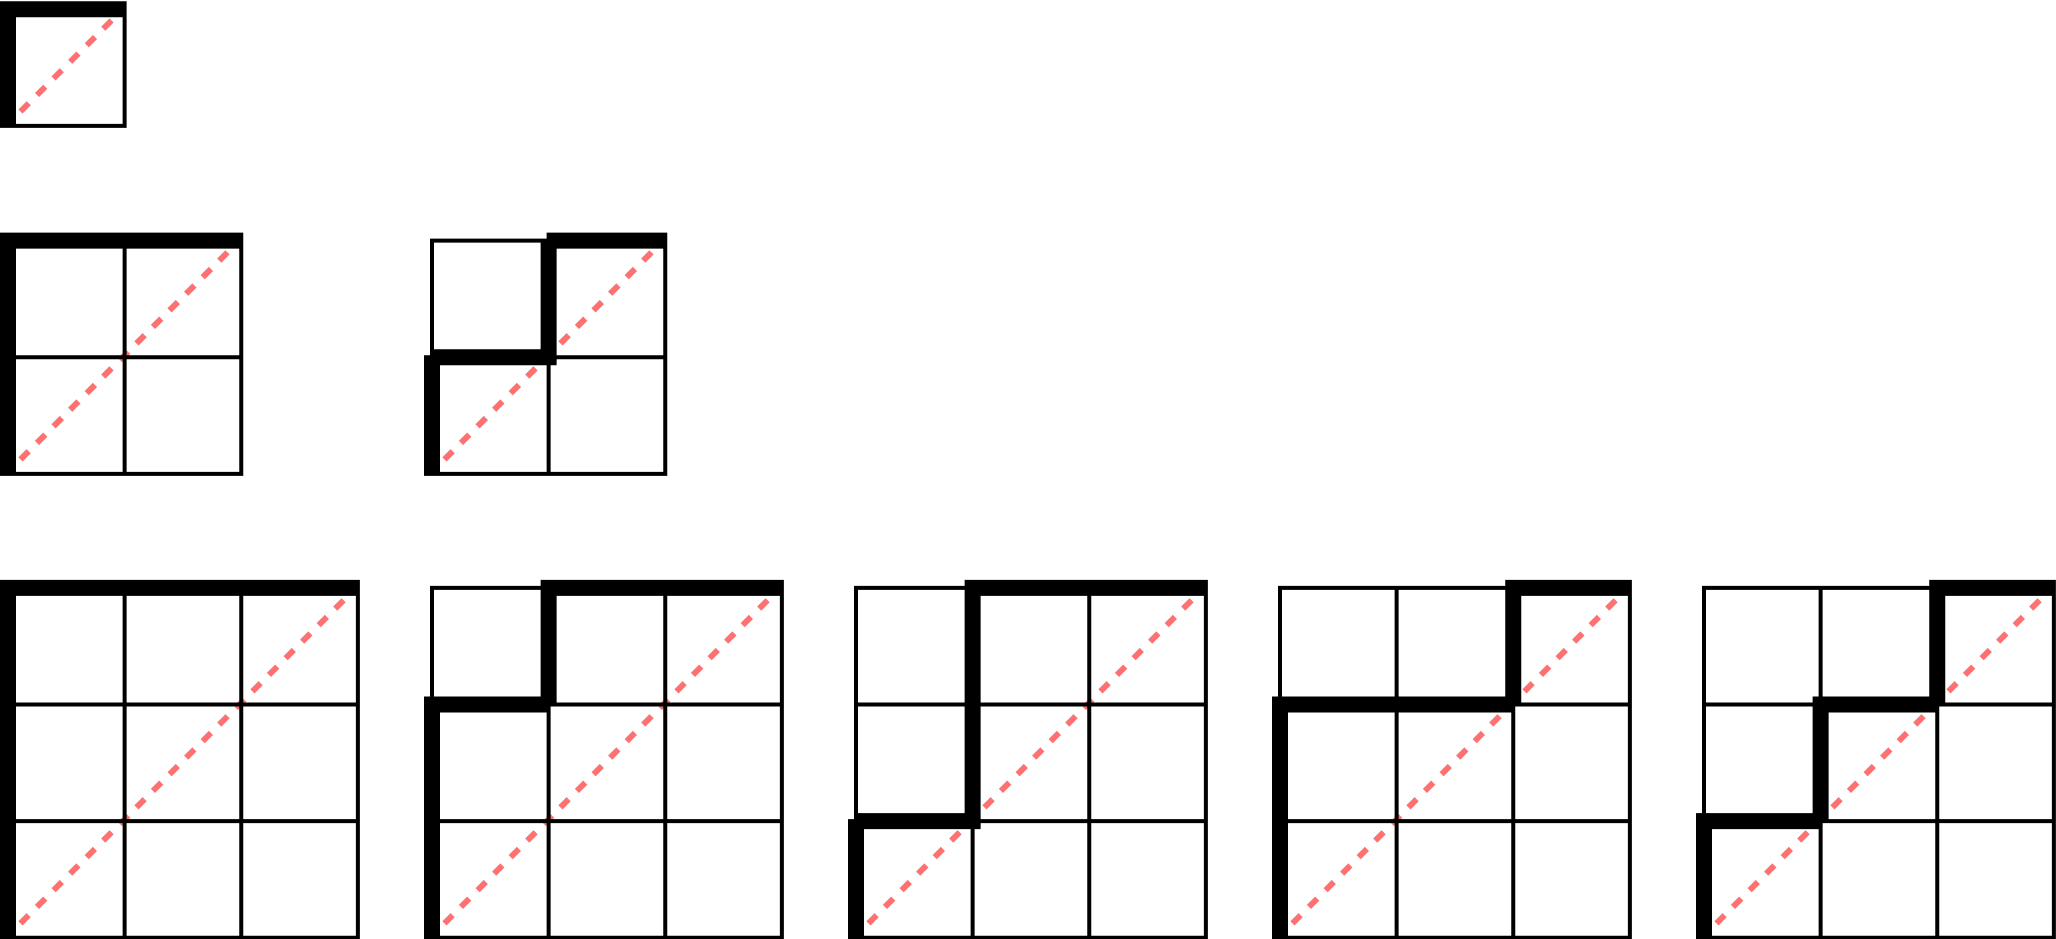
\includegraphics[width=0.8\linewidth]{Images/Figure11.png}
    \caption{All possible lattice paths which don't go below the diagonal for cases $n=1,2,3$}
    \label{f:3.21}
\end{figure}    
\begin{remark}
Notice that reflecting each path in \cref{f:3.21} across the main diagonal produces a lattice path that remains strictly below it. This bijection clearly shows that $a_1(n)$, the number of lattice paths that do not fall below the diagonal is the same as $a_2(n)$, the number of those that do not rise above it.
\end{remark}
\begin{question}
Count the number of ways $a_3(n)$, of filling a $2\times n$ grid with elements from the set $\{0,1,2,3,\cdots,2n\}$ such that all elements are unique, increasing row-wise, and decreasing column-wise.
\end{question}
\begin{solution}
\begin{figure}[H]
    \centering
    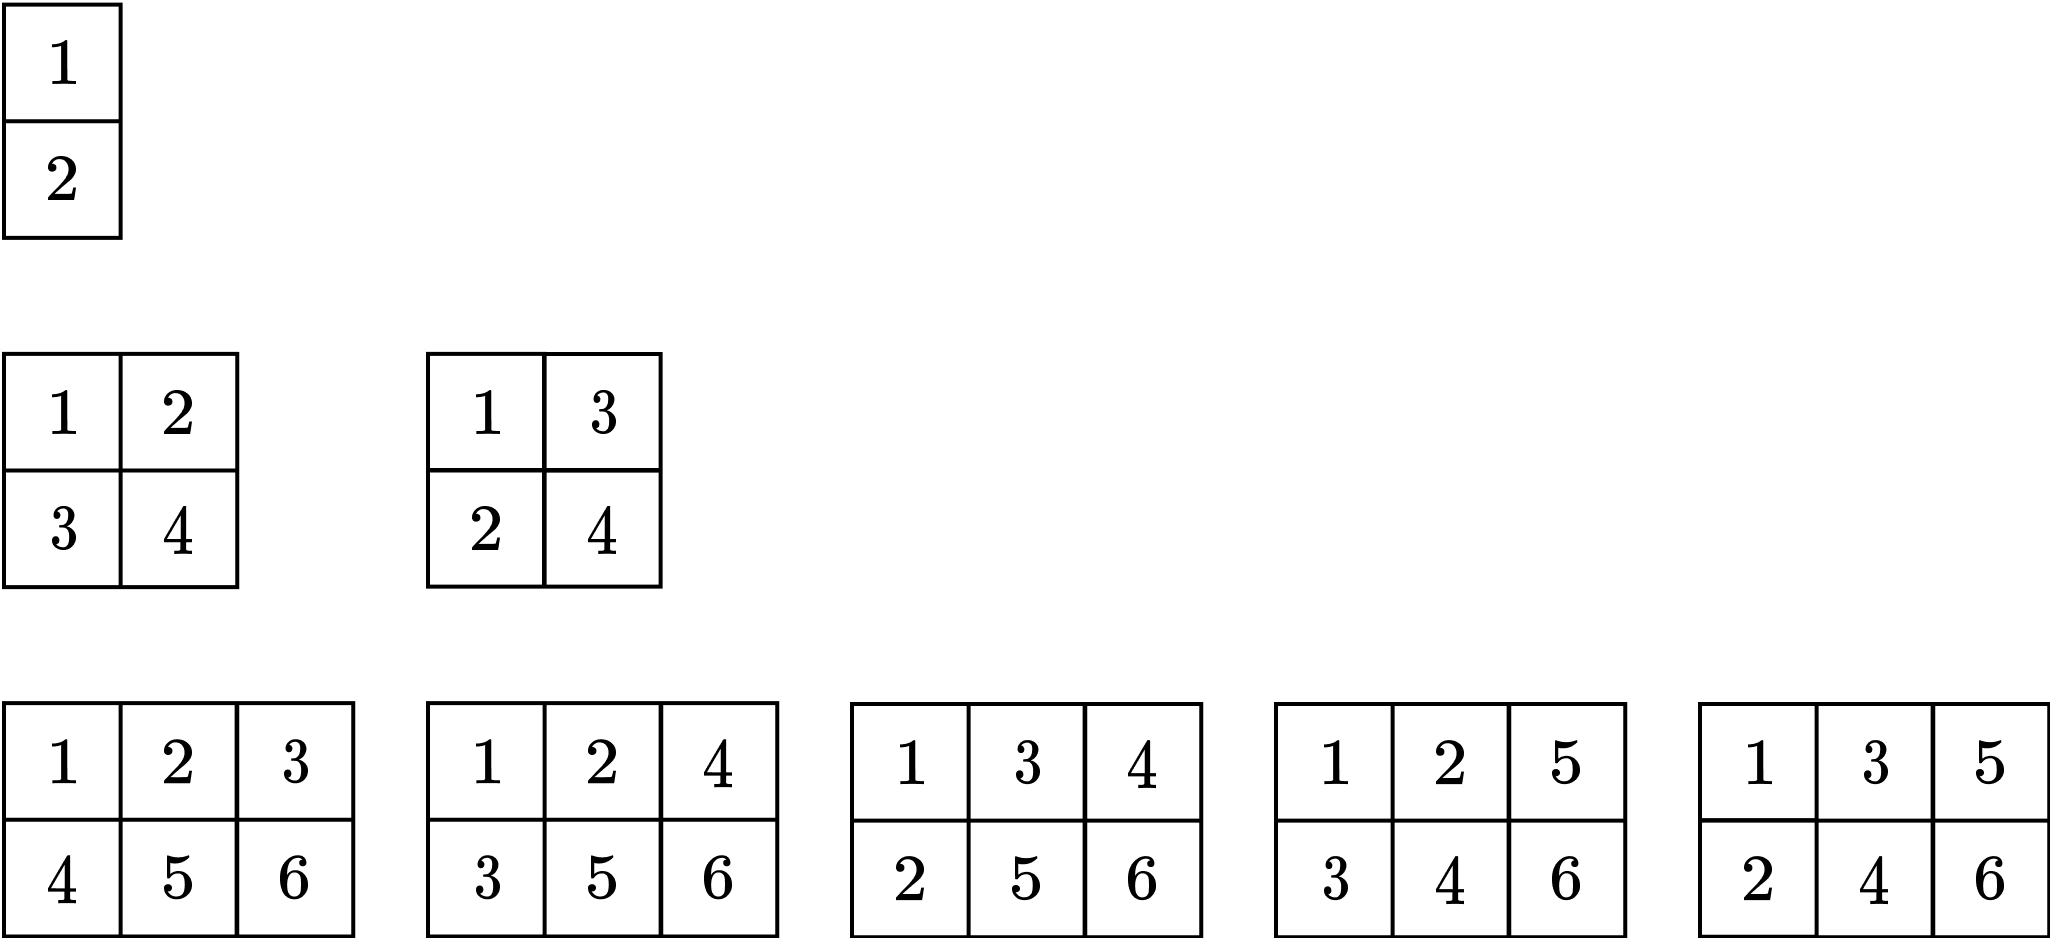
\includegraphics[width=0.8\linewidth]{Images/Figure12.png}
    \caption{All possible such arrangements of order $2\times n$ for cases $n=1,2,3$}
    \label{f:3.22}
\end{figure}
A bijection presents itself when \cref{f:3.21} and \cref{f:3.22} are compared. Namely, the entries in the first row of the $2\times n$ grid correspond to when an $N$-step in our lattice path occurs, and the entries in the second row correspond to when an $E$-step in our lattice path occurs.     
\end{solution}
\begin{question}
Count the number of Dyck paths $a_4(n)$, from $(0,0)$ to $(2n,0)$. Where, by a Dyck path we refer to the path admitted by a sequence of up-moves, corresponding to $(i,j)\to (i+1,j+1)$ and down-moves, corresponding to $(i,j)\to (i-1,j-1)$, which does not go below the $x$-axis.    
\end{question}
\begin{solution}
\begin{figure}[H]
    \centering
    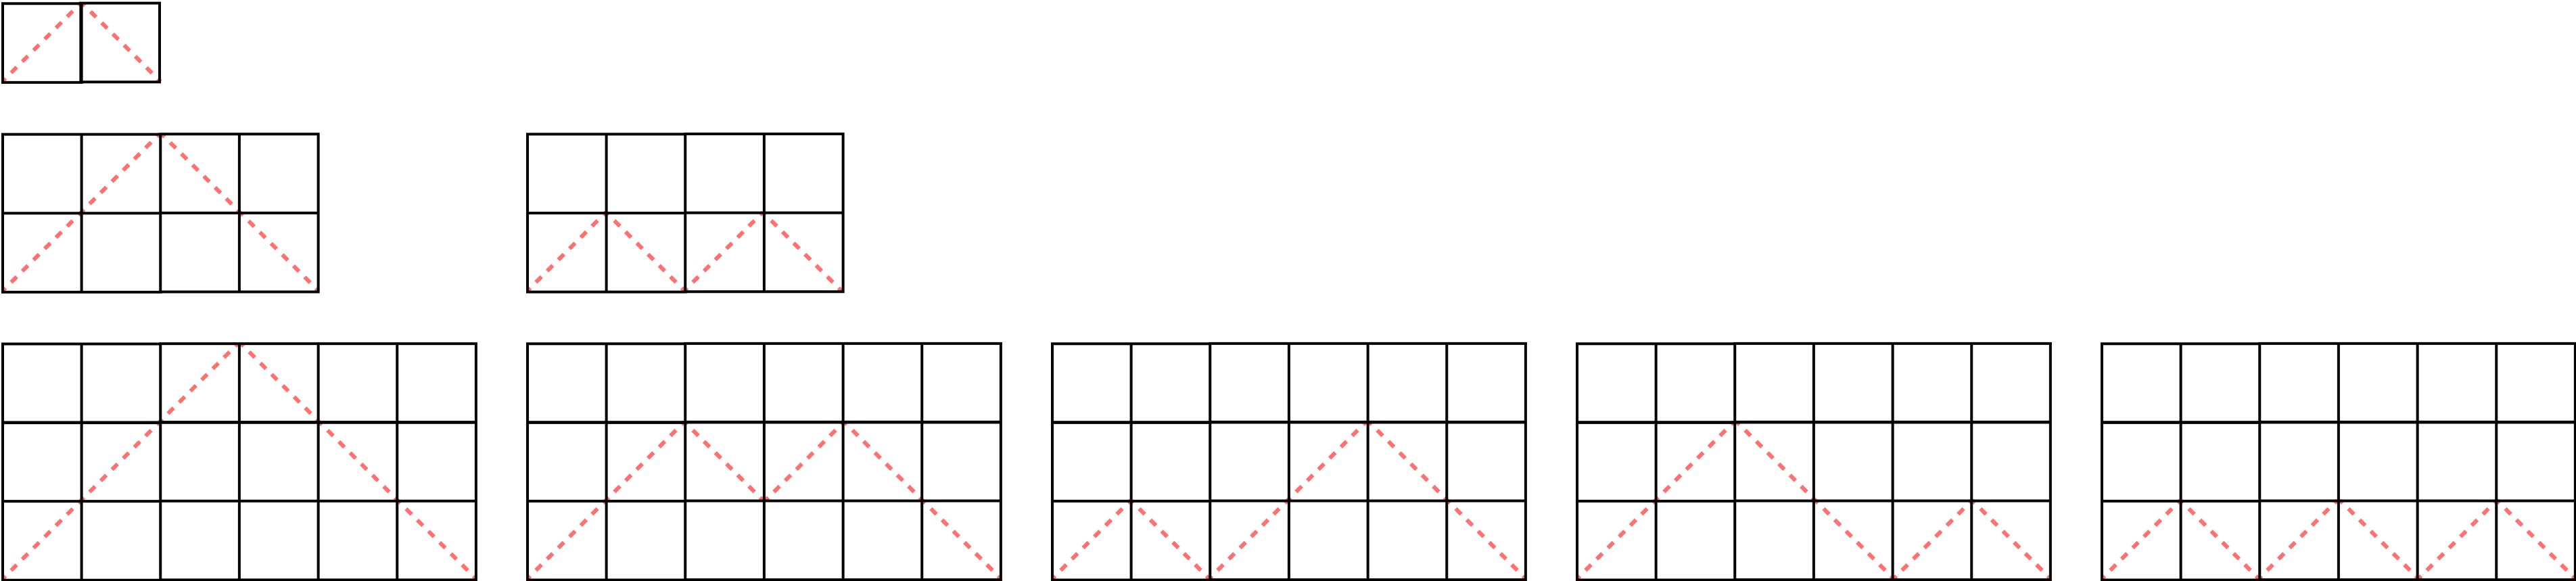
\includegraphics[width=1.2\linewidth]{Images/Figure13.png}
    \caption{All possible Dyck paths from  $(0,0)\to (2n,0)$ for $n=1,2,3$}
    \label{f:3.23}
\end{figure}
Once again, a bijection presents itself when \cref{f:3.21} and \cref{f:3.23} are compared. Namely, the entries in the first row of the $2\times n$ grid correspond to when an up-step in our Dyck path occurs, and the entries in the second row correspond to when a down-step in our Dyck path occurs.     
\end{solution}
\begin{question}
Count the number of ways $a_5(n)$, of joining $n$ non-intersecting chords on a circle marked with $2n$ points.     
\end{question}
\begin{solution}
\begin{figure}[H]
    \centering
    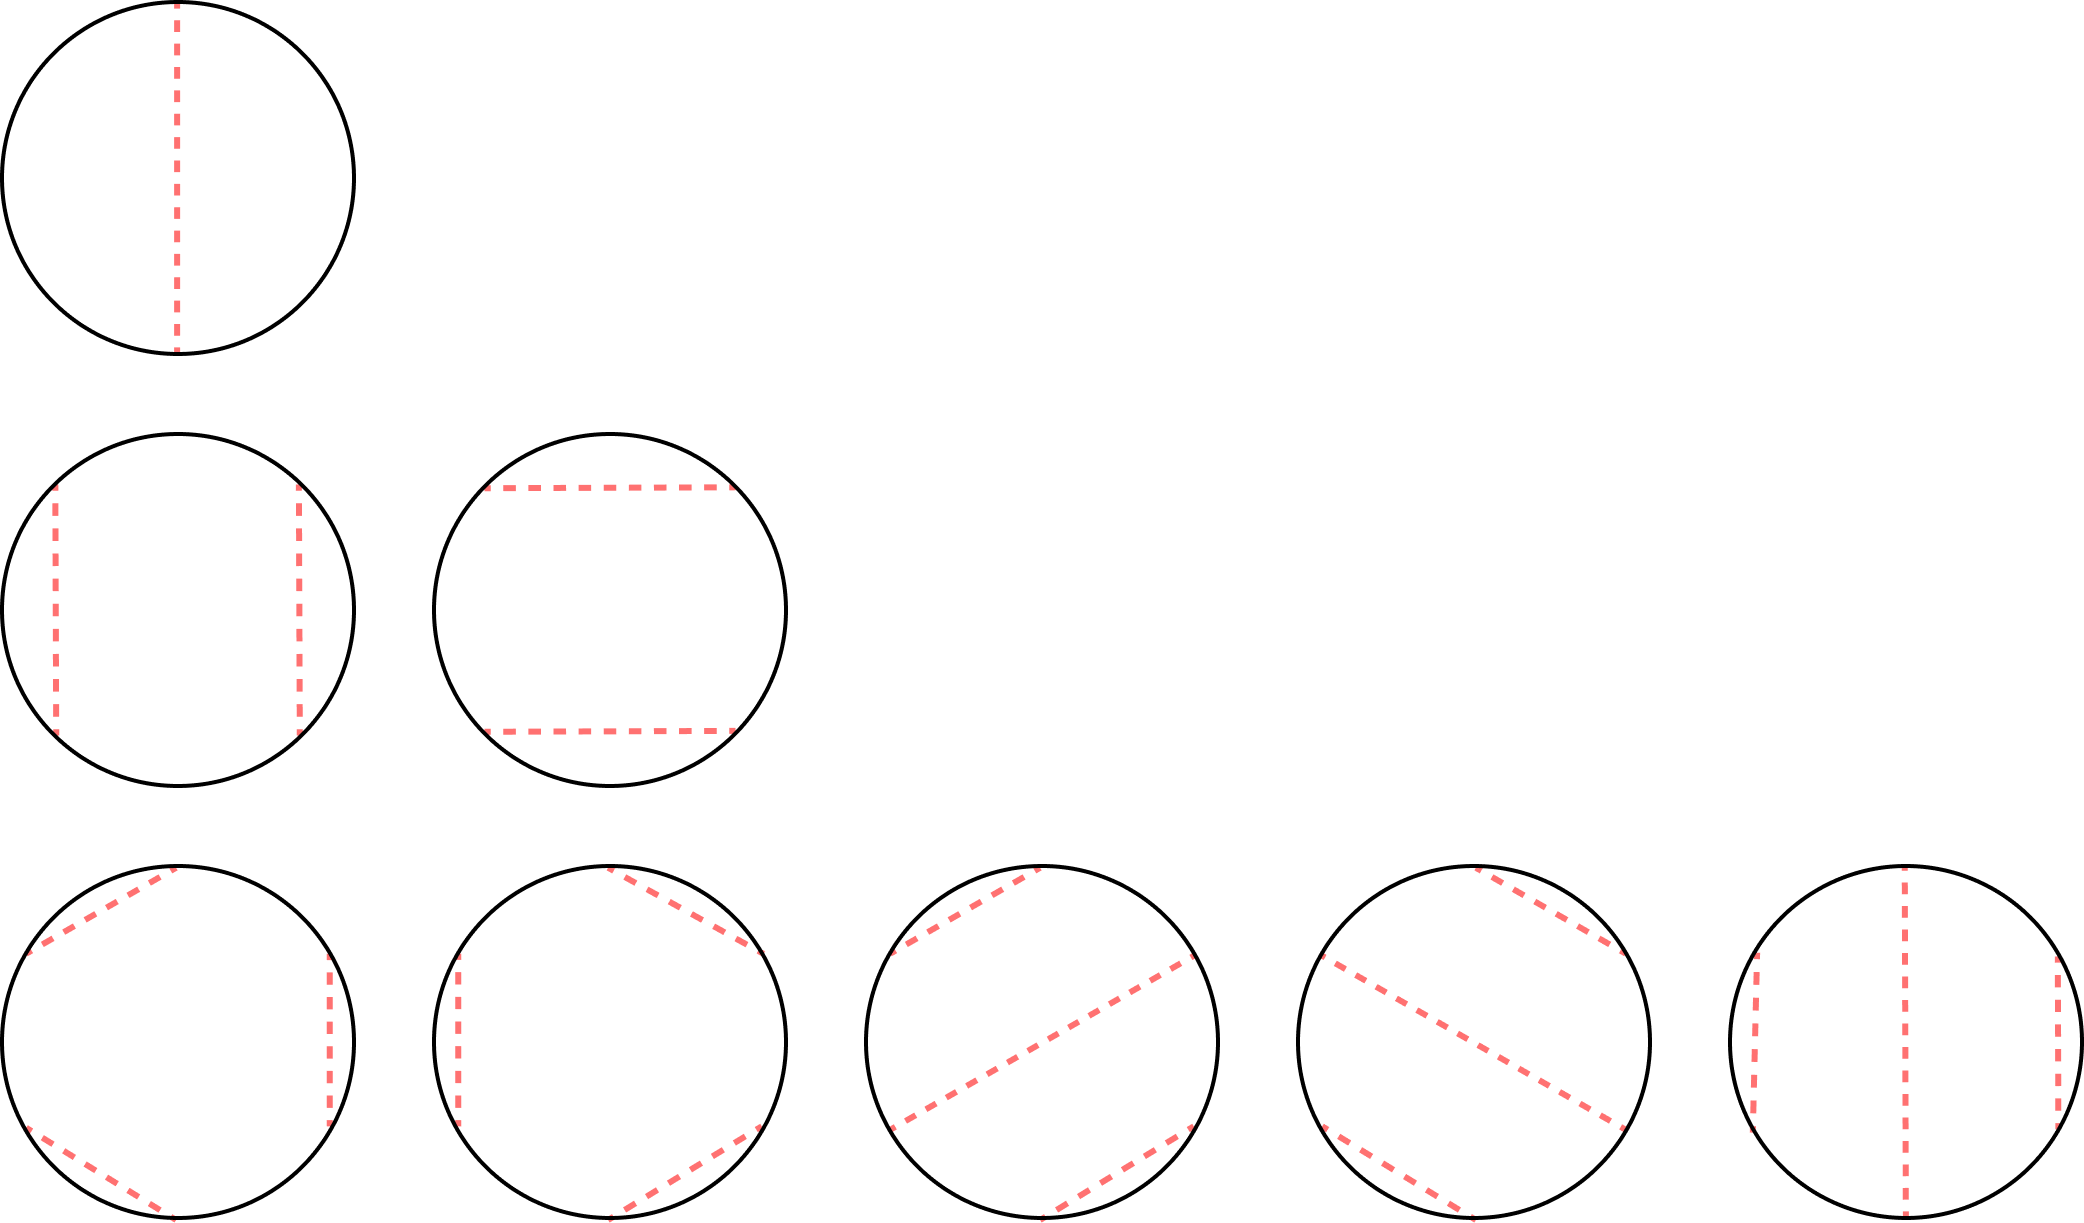
\includegraphics[width=0.8\linewidth]{Images/Figure14.png}
    \caption{All possible such configurations for cases $n=1,2,3$}
    \label{f:3.24}
\end{figure}
Once again, a bijection presents itself when \cref{f:3.22} and \cref{f:3.24} are compared. Namely, if $p_1,\cdots,p_{2n}$ are the marked points on the circle, then we join $p_i$ and $p_j$ if and only if $i$ occurs below $j$ in the arranged grid of numbers. 
\end{solution}
\begin{question}
Count $a_6(n)$, the number of legal sequences of $2n$ parentheses. Where, by a legal sequence of parentheses we mean one in which the parentheses can be properly matched, i.e, each opening parenthesis should be matched to a closing one that lies further to its right. We count these for $n=1,2,3$.
\begin{align*}
    & n=1: \quad \left(\right) \\
    & n=2: \quad \left(\left(\right)\right), \left(\right)\left(\right) \\
    & n=3: \quad \left(\left(\left(\right)\right)\right), \left(\right)\left(\left(\right)\right), \left(\left(\right)\right)\left(\right), \left(\right)\left(\right)\left(\right)
\end{align*}
Once again, notice how corresponding to each grid in \cref{f:3.22} there is a legal sequence of parentheses. Namely, for each entry in the first row we open a parenthesis, and close it for each entry in the second row.    
\end{question}
\begin{question}
Count $a_7(n)$, the number of non-crossing partitions on the set $[2n]:=\{1,2,3,\cdots,2n\}$. Where by a non-crossing partition on $[2n]$ we refer to an arrangement of $2n$ points on a line, with $n$ non-intersecting arcs joining them.    
\end{question}
\begin{solution}
\begin{figure}[H]
    \centering
    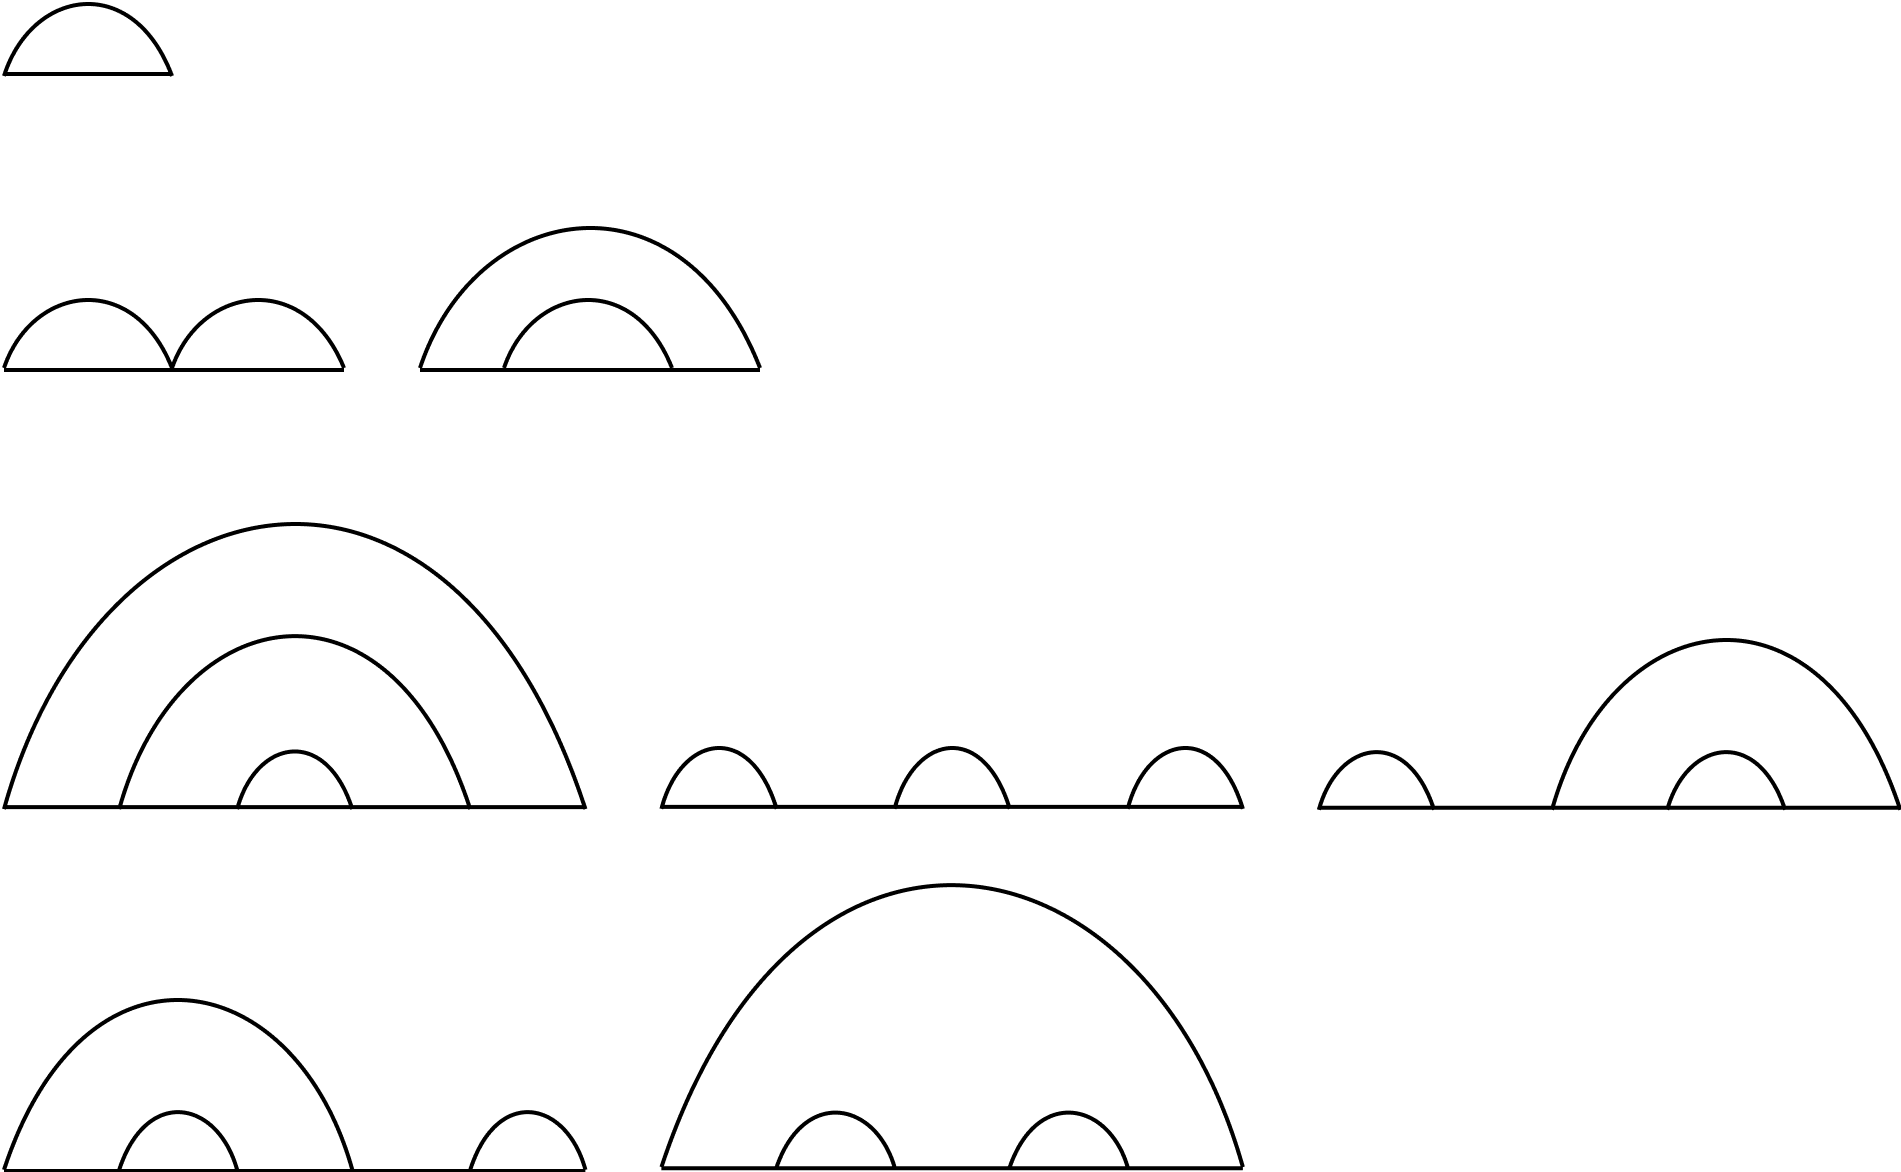
\includegraphics[width=0.8\linewidth]{Images/Figure15.png}
    \caption{All possible non-crossing partitions on $[2n]$ for $n=1,2,3$}
    \label{f:3.25}
\end{figure}
Once again, a bijection presents itself when \cref{f:3.22} and \cref{f:3.25} are compared. Namely, if $p_1,\cdots,p_{2n}$ are the marked points on the line, then we join $p_i$ and $p_j$ if and only if $i$ occurs below $j$ in the arranged grid of numbers. 
\end{solution}
To summarize, by the many bijections we have set up, $C(n):=a_1(n)=a_2(n)=\cdots=a_7(n)$ for all $n\geq 0$. Additionally, we have also seen that $A(n)$ takes values $1,1,2$ and $5$ for when $n=0,1,2$ and $3$ respectively. Motivated readers may check why and how $C(4)=14$, $C(5)=42$, and so on, but this is not how we want to proceed. Consider the following definitions.
\begin{definition}[Triangulation]
A triangulation of a convex polygon with $n+2$ vertices $\mathcal{P}_{n+2}$, is a set of $n-1$ diagonals which do not cross each other in the interior of $\mathcal{P}_{n+2}$. 
\end{definition}
\begin{remark}
For instance, the $3$-gon (triangle) has no triangulations, but the $4$-gon (square/rectangle) has $2$.    
\end{remark}
\begin{definition}[Catalan Numbers]
The sequence $C(n)$ which counts the the number of triangulations of $\mathcal{P}_{n+2}$ is called the sequence of Catalan numbers.
\label{d:catalan}
\end{definition}
\begin{theorem}
For all $n\geq 0$ we have
\[
C(n+1) = \sum_{k=0}^{n}C(k)C(n-k)
\]
\label{t:segner}
\end{theorem}
\begin{figure}[H]
    \centering
    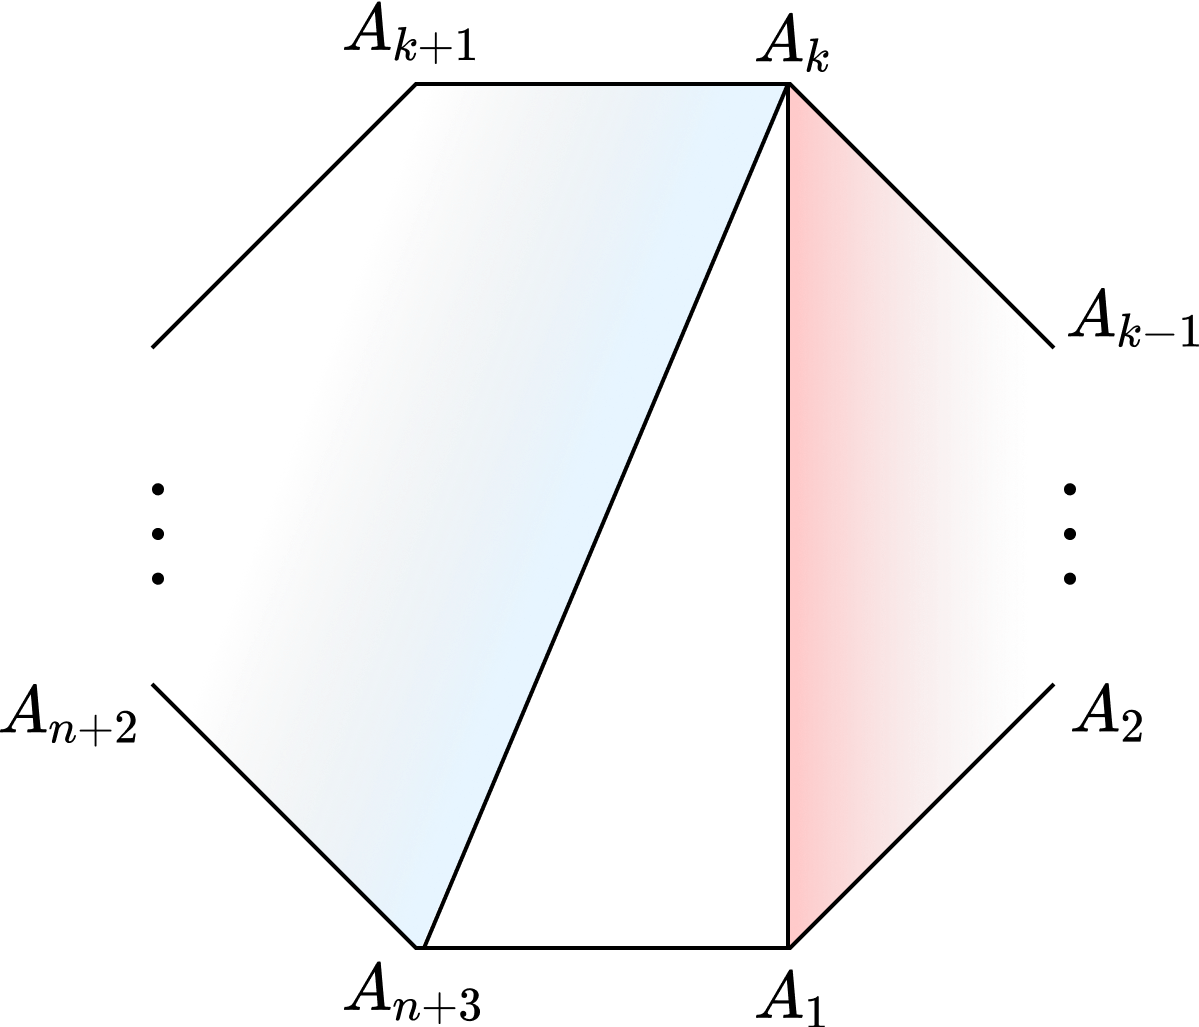
\includegraphics[width=0.45\linewidth]{Images/Figure16.png}
    \caption{}
    \label{f:3.26}
\end{figure}
\begin{proof}
Let $\mathcal{P}_{n+3}$ be an $n+3$ convex polygon with vertices $A_1,\cdots,A_{n+3}$. Next, pick an arbitrary vertex $A_k$ and consider the triangle $\Delta A_1A_{n+3}A_{k}$. See \cref{f:3.26} and notice how this choice splits $\mathcal{P}_{n+3}$ into two convex polygons. One with $k$ vertices (marked red) and the one with $n-k+4$ vertices (marked blue). Since $k$ is allowed to vary from $2$ to $n+2$, by \cref{d:catalan} we have $\sum_{k=2}^{n+2}C(k-2)C(n-k+2)$ ways to triangulate $\mathcal{P}_{n+3}$. Finally, shifting the index of summation by $2$ grants the required result. 
\end{proof}
\begin{claim}
\[
C(n) = \dfrac{1}{n+1}\binom{2n}{n}
\]
\end{claim}
\begin{proof}
Let \[f(x) = \sum_{n=0}^{\infty}C(n)x^n\] be the generating function corresponding to the Catalan numbers. By \cref{t:segner},
\begin{align*}
    f(x)^2 &= C(0)^2 + (C(0)C(1)+C(1)C(0))x + \cdots + (C(0)C(n)+C(1)C(n-1)+\cdots+C(n)C(0))x^n + \cdots \\
    &= C(1)+C(2)x+\cdots+C(n+1)x^n+\cdots \\
    &= \dfrac{C(x)-C(0)}{x}.
\end{align*}
Solving for $C(x)$ gives \[
C(x) = \dfrac{1\pm \sqrt{1-4x}}{2x}.
\]
Since $C(n)$ is always positive, we discard \[
C(x) = \dfrac{1+ \sqrt{1-4x}}{2x}.
\] and expand $\sqrt{1-4x}$ using \cref{t:2.3rev} to see why 
\[
C(x) = \sum_{n=0}^{\infty}\dfrac{1}{n+1}\binom{2n}{n}x^n.
\]
\end{proof}
\begin{remark}
Catalan numbers come up in a huge class of counting problems. In fact, Richard Stanley, in his book, ``Catalan Numbers'' outlines $214$ such problems. That being said, the many bijections we have outlined in this section are not always as easy to find. In such cases the defining recurrence (\cref{t:segner}) we have obtained is particularly useful. Consider the following example for instance.
\end{remark}
\begin{question}
Count the number of binary trees with $n$ vertices.
\end{question}
\begin{figure}[H]
    \centering
    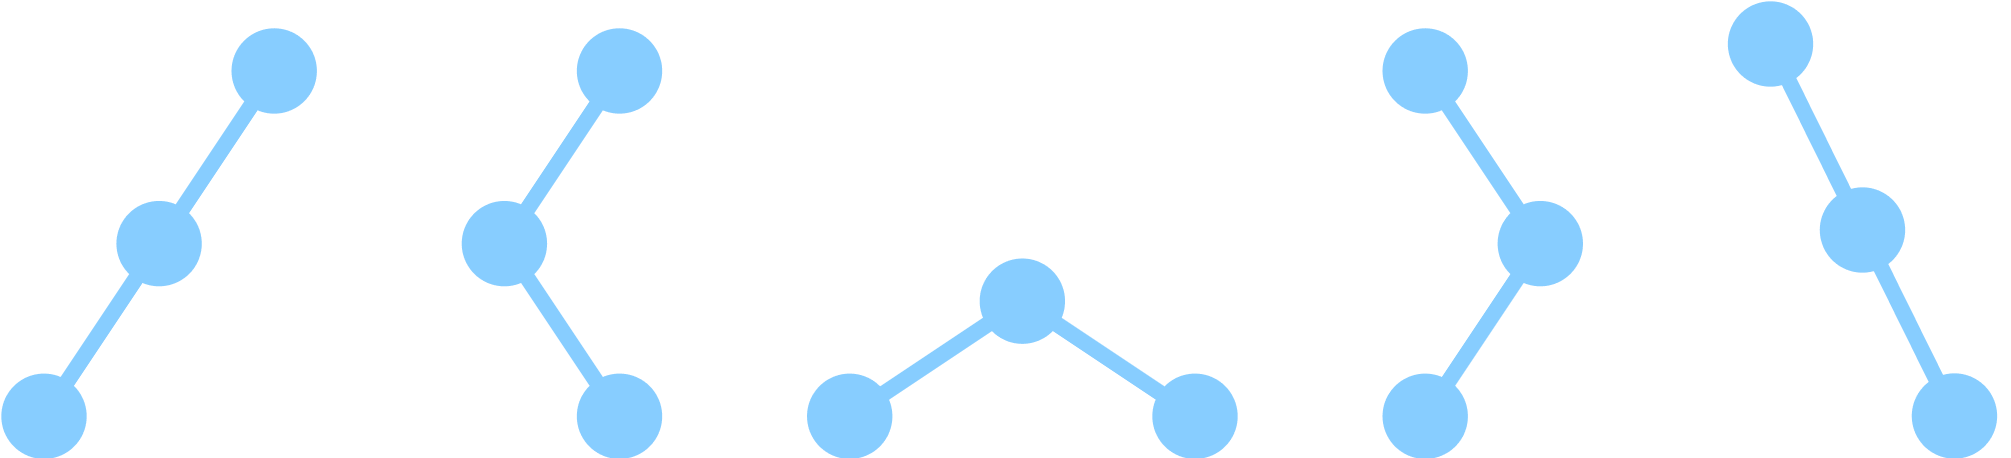
\includegraphics[width=0.7\linewidth]{Images/Figure23.png}
    \caption{The $5$ binary trees on $3$ vertices.}
\end{figure}
\begin{solution}
Let $a_n$ denote the number of binary trees with $n$ vertices, where $n\geq 0$. Since the empty tree is the only binary tree with $0$ vertices, it is clear why $a_0 = 1$. Similarly, it is also clear why $a_1=1$. Consider a binary tree $T$ (say) with $n$ vertices. The root of $T$ has $n-1$ children. For a choice of $0\leq i\leq n-i-1$ let $T$ have $i$ children on the left sub-tree and $n-i-1$ children on the right. By our set-up, there are $a_i$ binary trees with $i$ vertices and $a_{n-i-1}$ binary trees with $n-i-1$ vertices. It follows that there are $a_i a_{n-i-1}$ binary trees with $i$ children on their left subtrees and $n-i-1$ children on their right. Thus, the total number of binary trees with $n$ vertices is given by
\[
a_n = \sum_{i=0}^{n-1}a_ia_{n-i-1}.
\]
Comparing with \cref{t:segner} we get that $a_n$ is counted by the Catalan numbers. 
\end{solution}
We are now interested in stating a recurrence for Catalan numbers which is different from the one we already stated. To this end consider the following theorem and it's corollary. 
\begin{theorem}
    Let $T_n$ be the number of triangulations of an $n$-gon, then for $n\geq 4$,
    \[
    (2n-6)T_n = n\sum_{k=3}^{n-1}T_kT_{n-k+2}
    \]
\end{theorem}
\begin{figure}[H]
    \centering
    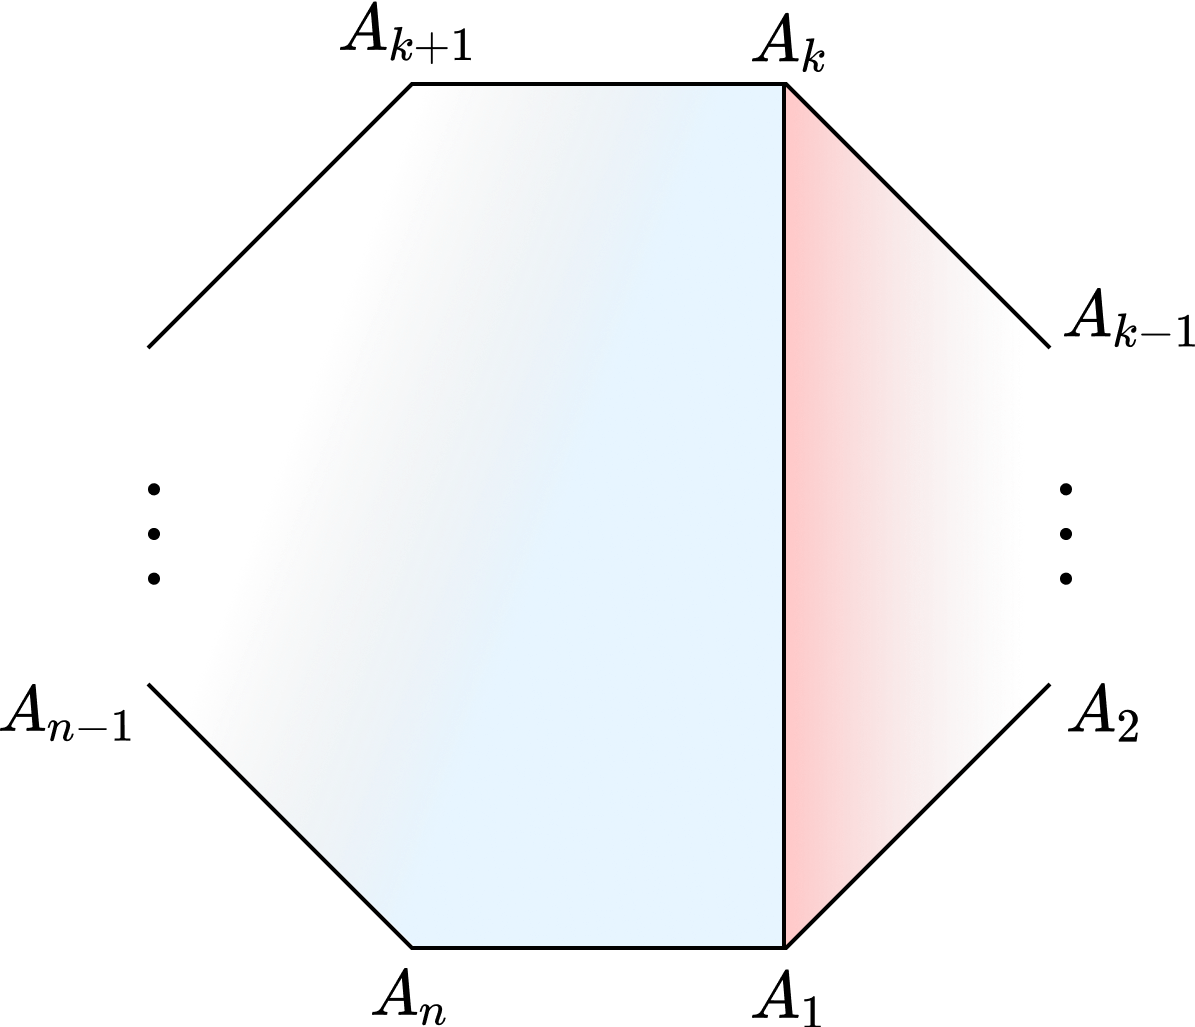
\includegraphics[width=0.45\linewidth]{Images/Figure22.png}
    \caption{}
    \label{f:Segner2f}
\end{figure}
\begin{proof}
Consider an $n$-gon with vertices $A_1,A_2,\ldots,A_n$. Conisder an arbitrary diagonal $\overline{A_1A_k}$ leaving $A_1$, where $2<k<n$. See \cref{f:Segner2f} and notice how this partitions the $n$-gon into the $k$-gon $A_1A_2\ldots A_k$ (marked red) and the $(n-k+2)$-gon $A_1A_kA_{k+1}\ldots A_n$ (marked blue). The $k$-gon can be triangulated in $T_k$ ways and the $(n-k+2)$-gon in $T_{n-k+2}$ ways. It follows that the $n$-gon can be triangulated in a total of $T_kT_{n-k+2}$ ways. Since $k$ is allowed to vary between $3$ and $n-1$, it also follows that the total number of triangulation based at $A_1$ are given by \[
\sum_{k=3}^{n-1}T_kT_{n-k+2}.
\]
Our choice of $A_1$ is not special. Since there $n$ choices of vertices where the triangulation can be based one might think the count is
\[
n\sum_{k=3}^{n-1}T_kT_{n-k+2}.
\]
However, we have overcounted. More specifically, the diagonals $\overline{A_iA_j}$ are counted twice. This gives;
\[
n/2\sum_{k=3}^{n-1}T_kT_{n-k+2}.
\]
Finally, since the $n$-gon has $n-3$ diagonals at every vertex and every triangulation uses $n-3$ diagonals, it follows that
\[
(n-3)T_n = n/2\sum_{k=3}^{n-1}T_kT_{n-k+2}.
\]
as required.
\end{proof}
A corollary follows naturally.
\begin{corollary}
\[
(2n-2)C_n = (n+2)\sum_{k=1}^{n-1}C_kC_{n-k}
\]
\end{corollary}
\chapter{Generating Functions}
This chapter builds on our earlier discussion of generating functions from Chapter 1 (see \cref{d:1.4}). Among the various types used in combinatorics and other fields like number theory, we will focus on two: ordinary generating functions and exponential generating functions
\section{Ordinary Generating Functions}
We start with a few examples.
\begin{example}
Corresponding to the constant sequence of $1$s, the generating function is $1+x+x^2+x^3+\cdots = \dfrac{1}{1-x}$
\end{example}
\begin{example}
Corresponding to the sequence $1,2,3,\cdots$, the generating function is $1+2x+3x^2+4x^3+\cdots = 1/(1-x)^2$. Notice how equality follows from the fact that $1+2x+3x^2+4x^3+\cdots$ is the formal derivative of the generating function we obtained in the previous example.
\end{example}
More often than not generating functions are used to solve recurrences. For instance consider the following question.
\begin{question}
Find a closed form expression for the recurrence given by $a_{n+1}=2a_n+1$ where $a_0=0$. 
\end{question}
\begin{solution}
Let $A(x)=a_0+a_1x+a_2x^2+\cdots$ be the generating function corresponding to the sequence. Notice how 
\begin{align*}
    &\sum_{n\geq 0}a_{n+1}x^n = 2\sum_{n\geq 0}a_nx^n+ \sum_{n\geq 0}x^n \\
    &\implies \dfrac{A(x)}{x} = 2A(x) + \dfrac{1}{1-x} \\
    &\implies A(x) = \dfrac{x}{(1-x)(1-2x)} \\
    &\implies A(x) = \dfrac{1}{1-2x}-\dfrac{1}{1-x} \\
    &\implies A(x) = (1+2x+4x^2+8x^3+\cdots)-(1+x+x^2+x^3+\cdots) \\
    &\implies A(x) = x+3x^2+7x^3+\cdots
\end{align*}
Now $a_n$ is just the coefficient of $x^n$ in $A(x)$. 
\end{solution}
We state one more example. Recall how with \cref{q:1.9}, we found the generating function for the sequence of Fibonacci numbers. We are now interested in finding a closed form of numbers in this sequence. 
\begin{solution}
Let $r_1,r_2 = (-1\pm\sqrt{5})/2$ be the roots of the polynomial $1-x-x^2$ and notice how
\begin{align*}
    F(x) &= \dfrac{1}{1-x-x^2} \\
    &= \dfrac{1}{(r_1-x)(r_2-x)} \\
    &= \dfrac{1}{(r_1-x)(r_2-r_1)}+\dfrac{1}{(r_2-x)(r_1-r_2)} \\
    &= \dfrac{1}{\sqrt{5}}\left(\dfrac{1}{r_2-x}-\dfrac{1}{r_1-x}\right) \\
    &= \dfrac{1}{\sqrt{5}} \left(\dfrac{1/r_2}{1-(x/r_2)}-\dfrac{1/r_1}{1-(x/r_1)}\right) \\
    &= \dfrac{1}{\sqrt{5}} \left(\dfrac{1}{r_2}\left(1+\dfrac{x}{r_2}+\dfrac{x^2}{r_2^2}+\cdots\right)-\dfrac{1}{r_1}\left(1+\dfrac{x}{r_1}+\dfrac{x^2}{r_1^2}+\cdots\right)\right) \\
    &= \dfrac{1}{\sqrt{5}}\left(\dfrac{1}{r_2}+\dfrac{x}{r_2^2}+\dfrac{x^2}{r_2^3}+\cdots - \dfrac{1}{r_1}-\dfrac{x}{r_1^2}-\dfrac{x^2}{r_1^3}-\cdots\right) \\
    &= \dfrac{1}{\sqrt{5}}\left(\left(\dfrac{1}{r_2}-\dfrac{1}{r_1}\right)+\left(\dfrac{1}{r_2^2}-\dfrac{1}{r_1^2}\right)x+\left(\dfrac{1}{r_2^3}-\dfrac{1}{r_1^3}\right)x^2+\cdots\right)
\end{align*}
Now, the $n$-th Fibbonaci number is just the coefficient of $x^n$ in $F(x)$. 
\end{solution}
Often-times we are interested in computing the product of two generating functions. To this end,consider the following result due to Cauchy. 
\begin{claim}[Cauchy Product]
Let $A(x) = \sum_{n\geq 0}a_nx^n$ and $B(x)=\sum_{n\geq 0}b_nx^n$ be two ordinary generating functions. Their product $C(x)$, is then given by $A(x)B(x)=\sum_{n\geq 0}c_nx^n$ where \[
c_n = \sum_{k=0}^{n}a_kb_{n-k}
\]
\end{claim}
\section{Exponential Generating Functions}
\endinput

\chapter{Integer Partitions}







\endinput

\chapter{Lattice Path Combinatorics}



\section{Dyck Paths Revisited}

\section{Motzkin and Schr\"oder Paths}


\section{Non-intersecting lattice paths}


\section{\texorpdfstring{$q-$} CCounting of lattice paths}


\endinput


\chapter{A Combinatorial Miscellany}


%\section{Domino Tilings}


%\section{Permutations}

\section{Perfect Matchings and Pfaffian Orientations}
Refer to \href{https://youtu.be/ydCWu6aiAxE?si=v91XmPDjM3qkfGKw}{https://youtu.be/ydCWu6aiAxE?si=v91XmPDjM3qkfGKw}. 
\section{Graphs and Trees}
We start with a standard result on graphs.
\begin{theorem}
    Let $G$ be a simple, connected graph on $n$ vertices. Then the following are equivalent.
    \begin{enumerate}
        \item $G$ is minimally connected.
        \item $G$ has $n-1$ edges.
        \item $G$ has no cycles.
    \end{enumerate}
    \label{t:G&T_Main}
\end{theorem}
\begin{proof}
If $G$ is minimally connected, then removing any edge of $G$ would disconnect it. This means that each edge of $G$ is a bridge. Since G is connected, it must have at least $n-1$ edges. If G had more than $n-1$ edges, then removing any additional edge would not disconnect $G$, contradicting the minimality assumption. Therefore, $G$ must have exactly $n-1$ edges. This proves that $(1)\implies (2)$. If G has $n-1$ edges and $n$ vertices, then it is a tree. Trees are acyclic by definition, so $G$ has no cycles. This proves $(2)\implies (3)$. Finally, if G has no cycles, then it is a tree. Trees are minimally connected, meaning that removing any edge disconnects the graph. Therefore, $G$ is minimally connected. This proves $(3)\implies (1)$. Having formed a loop of implications, we are done.
\end{proof}
Recall the following definitions. Graphs satisfying any one of the properties in \cref{t:G&T_Main} are called trees. Additionally, graphs whose connected components are trees are called forests. More importantly, a tree on $n$ vertices is called a labeled tree if each vertex gets a label from the set $[n]$. 
\par
With this background at hand, we are interested in counting $T_n$, the number of labeled trees on $n$ vertices. From the figure below it is clear that $T_1,T_2,T_3$ and $T_4$ are $1,1,3$ and $16$. One might guess that $T_n=n^{n-2}$. In fact this is precisely what we want to prove.
\begin{figure}[H]
    \centering
    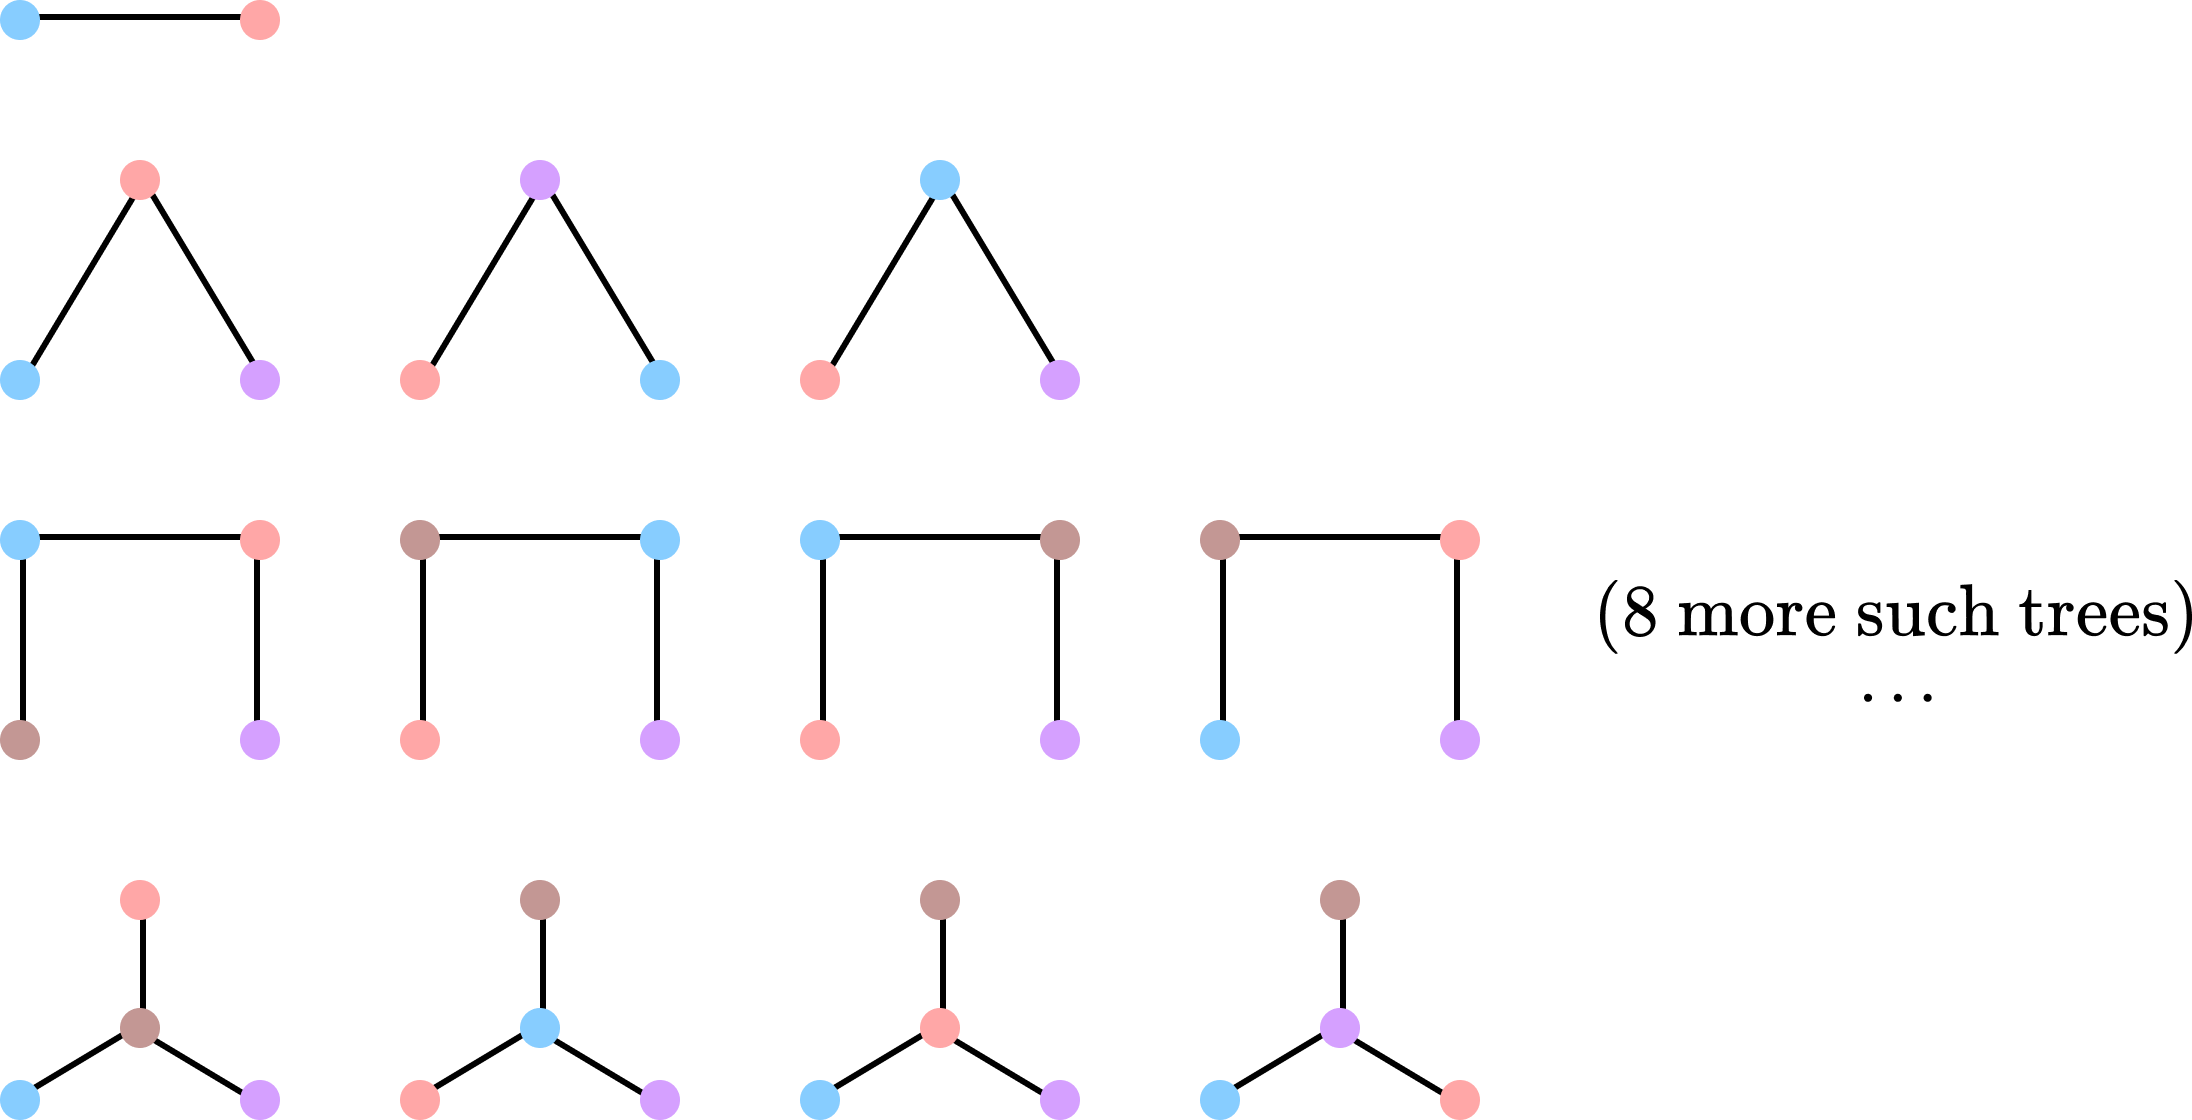
\includegraphics[width=0.9\linewidth]{Images/Figure29.png}
    \caption{}
    \label{f:Cayley Trees}
\end{figure}

\begin{theorem}[Cayley's Formula]
If $T_n$ denotes the number of labeled trees on $n$ vertices, then
    \[
    T_n = n^{n-2}.
    \]
    \label{t:Cayley's Formula}
\end{theorem}
\begin{proof}
Let $A=[k]$ be a set of vertices. Let $T_{n,k}$ count the number of labeled forests on $[n]$ consisting of $k$ trees where the vertices of $A$ appear in different trees. Let $F$ be a forest in this setting.
\begin{figure}[H]
    \centering
    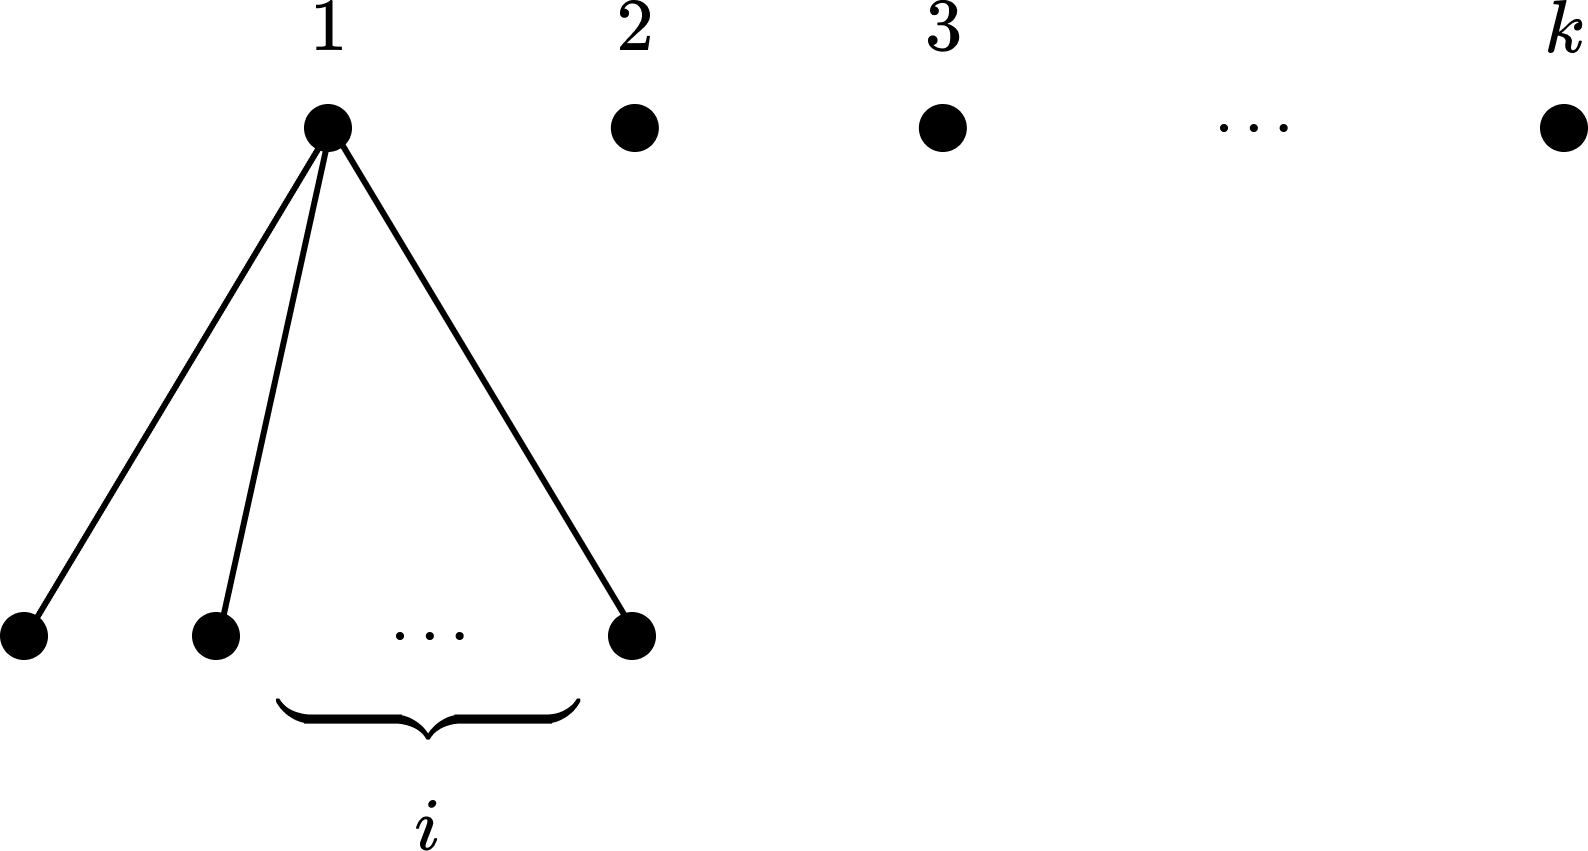
\includegraphics[width=0.5\linewidth]{Images/Figure30.png}
    \caption{}
    \label{f:CTProof}
\end{figure}
As is clear by \cref{f:CTProof}, if $1$ is adjacent to $i$ vertices, deleting it, the $i$ neighbors together with $2,\ldots,k$ yield one vertex each in the components of a forest that consists of $k-1+i$ trees. Since $F$ can also be constructed by fixing $i$, then choosing the $i$ neighbors of $1$ and then the forest $F\backslash \{1\}$ gives \[
T_{n,k} = \sum_{i=0}^{n-k}\binom{n-k}{i}T_{n-1,k-1+i}
\]
for all choices of $n\geq k\geq 1$ where $T_{0,0}=1$ and $T_{n,0}=0$ as expected. By induction and the expression for $T_{n,k}$ which we have found, it follows that
\begin{align*}
    T_{n,k}&= \sum_{i=0}^{n-k}\binom{n-k}{i}(k-1+i)(n-1)^{n-1-k-i} \\
    &= \sum_{i=0}^{n-k}(n-1)^i-\sum_{i=1}^{n-k}\binom{n-k}{i}i(n-1)^{i-1} \\
    &= n^{n-k}-(n-k)\sum_{i=0}^{n-1-k}\binom{n-1-k}{i}(n-1)^i \\
    &= n^{n-k}-(n-k)n^{n-1-k} \\
    &= kn^{n-1-k}.
\end{align*}
Setting $k\to 1$ gives us the required result.
\end{proof}
\begin{theorem}
The number of rooted forests on $[n]$ is $(n+1)^{n-1}$.
\end{theorem}
\begin{proof}
The proof follows from the following observation. For any rooted forest with \( n \) vertices, add a new vertex \( v \) and connect it to all the roots as their parent. This forms a tree with \( n + 1 \) vertices. Conversely, for any tree with \( n + 1 \) vertices, where one vertex is labeled \( v \), remove \( v \) along with its edges. The resulting structure is a rooted forest, with the former children of \( v \) serving as the roots.
\end{proof}
We conclude this section with a result whose proof we shall omit but see \cref{t:Cayley's Formula} as a consequence of. 
\begin{theorem}
    The number of rooted forests on $[n]$ with $k$ components is \[
    \binom{n-1}{k-1}n^{n-k}.
    \]
\end{theorem}
Notice how setting $k\to 1$ and multiplying the result by $n$ (to account for the $n$ choices of roots) gives \cref{t:Cayley's Formula} back. 
\section{Permutations Revisited}
We are interested in counting \( P_n \), the number of permutations on \([n]\) that can be generated using a single stack. We start by computing $P_n$ by hand for $n=1,2$ and $3$. When $n=1$, we can push $1$ on to the empty stack and pop it immediately. The stack is now empty, and there are no more input values. So we are done and the output is the permutation $(1)$. Next, when $n=2$, we have two possible permutations, $(12)$ and $(21)$. To obtain the permutation $(12)$, first push $1$ onto the stack, then pop it, then push $2$ onto the stack and then pop it. To obtain the permutation $(21)$, first push $1$ onto the stack, then push $2$, then pop $2$, and then pop $1$. Similarly, the permutations $(123),(132),(213),(231)$ and $(321)$ are obtainable. One might (correctly) guess from here one that this is the sequence of Catalan numbers. What follows is a proof of the same.
\begin{proof}
To this end, let \( i \) denote the position of the element \( 1 \) in a valid permutation produced by the stack, where \( 1 \leq i \leq n \). Then, \( P_{i-1} \) counts the number of valid permutations with \( i-1 \) elements to the left of \( 1 \), and \( P_{n-i-1} \) counts the number of valid permutations with \( n-i-1 \) elements to the right of \( 1 \). If we set \( P_0 = 1 \), then by the multiplication and addition principles, we obtain the recurrence
\[
P_n = \sum_{i=1}^n P_{i-1} P_{n-i-1},
\]
which, more explicitly is written as 
\[
P_n = P_0 P_{n-1} + P_1 P_{n-2} + \cdots + P_{n-1} P_0.
\]
Recall how this is precisely the recurrence relation we derived in \cref{t:segner}. Therefore, \( P_n = C_n \) for all \( n \geq 0 \), where \( C_n \) denotes the \( n \)-th Catalan number.
\end{proof}
\endinput


\backmatter
%%-----------------------------------------------------------------------------
% Beginning of biblio.tex
%-----------------------------------------------------------------------------

\bibliographystyle{amsalpha}
\begin{thebibliography}{A}

\bibitem [A]{A} T. Aoki, \textit{Calcul exponentiel des op\'erateurs
microdifferentiels d'ordre infini.} I, Ann. Inst. Fourier (Grenoble)
\textbf{33} (1983), 227--250.

\bibitem [B]{B} R. Brown, \textit{On a conjecture of Dirichlet},
Amer. Math. Soc., Providence, RI, 1993.

\bibitem [D]{D} R. A. DeVore, \textit{Approximation of functions},
Proc. Sympos. Appl. Math., vol. 36,
Amer. Math. Soc., Providence, RI, 1986, pp. 34--56.

\end{thebibliography}

%-----------------------------------------------------------------------------
% End of biblio.tex
%-----------------------------------------------------------------------------

\end{document}
